\documentclass[a4paper, twoside, 11pt, spanish]{book}

%% Paquetes
\usepackage[es-tabla]{babel}
\usepackage{amsmath, amsfonts, amssymb, amsthm}
\usepackage{color, graphicx, rotating, subcaption}
\usepackage[margin=2.2cm]{geometry}
\usepackage{hyperref, url}
\usepackage[font=small, labelfont=bf]{caption}
\usepackage{enumerate, enumitem}
\usepackage{tabularx}
\usepackage{ctable}
\usepackage{multicol}
\usepackage{float}
\usepackage{listings}
\usepackage[utf8]{inputenc}
\usepackage{longtable}
\usepackage{xcolor}
\usepackage{adjustbox}
\usepackage[square,numbers,sort&compress]{natbib}

\renewcommand{\baselinestretch}{1.2} % interlineado
\decimalpoint{} % cambia coma por punto

\DeclareMathOperator*{\argmax}{arg\,max}
\DeclareMathOperator*{\argmin}{arg\,min}

\theoremstyle{definition}
\newtheorem{theorem}{Teorema}[chapter]
\newtheorem{lemma}[theorem]{Lema}
\newtheorem{corollary}[theorem]{Corolario}
\newtheorem{remark}{Observaci\'on}[chapter]
\newtheorem{definition}{Definici\'on}[chapter]
\newtheorem{remarkex}{Observaci\'on}[chapter]

% Default fixed font does not support bold face
\DeclareFixedFont{\ttb}{T1}{txtt}{bx}{n}{12} % for bold
\DeclareFixedFont{\ttm}{T1}{txtt}{m}{n}{12}  % for normal

% Custom colors
\usepackage{color}
\definecolor{deepblue}{rgb}{0,0,0.5}
\definecolor{deepred}{rgb}{0.6,0,0}
\definecolor{deepgreen}{rgb}{0,0.5,0}

% Python style for highlighting
\newcommand\pythonstyle{\lstset{
    language=Python,
    basicstyle=\ttfamily\small,
    keywordstyle=\color{blue}\bfseries,
    stringstyle=\color{red}\ttfamily,
    commentstyle=\color{green}\ttfamily,
    showstringspaces=false,
    frame=single,
    breaklines=true,
    breakatwhitespace=false,
    backgroundcolor=\color{gray!10}
}}

% Python environment
\lstnewenvironment{python}[1][]
{\pythonstyle\lstset{#1}}
{}

%% Bibliografía
\bibliographystyle{unsrtnat}
\addto{\captionsspanish}{\renewcommand{\bibname}{Referencias}}

%% Tablas
\renewcommand{\tablename}{Tabla}
\renewcommand{\contentsname}{Índice}

% Encabezados y pies de pagina solo con numero de pagina
\pagestyle{plain}

\begin{document}
 
\frontmatter

% Caratula
\newgeometry{top=5cm,bottom=2cm,left=3cm,right=3cm}
%%
%% Caratula de la tesis
%%
\thispagestyle{empty}

\begin{center}
  
\includegraphics[scale = 0.3]{logofac.jpg}
  
  \medskip
  UNIVERSIDAD DE BUENOS AIRES
  
  Facultad de Ciencias Exactas y Naturales
  
 
  
  \vspace{3cm}
  \textbf{\large Estimación por intervalos de las proporciones de clases en muestras sin etiquetar utilizando la distribución Poisson-Binomial}
  
  \vspace{2cm}
  Tesis presentada para optar al título de Magister en Estadística Matemática de
  la Universidad de Buenos Aires
  
  \vspace{2cm}
  \textbf{Ing. Maximiliano Marufo da Silva}
\end{center}


\vspace{1.5cm}
\noindent Director de tesis: Dr.~Andrés Farall
 

\vspace{1cm}
\noindent Buenos Aires,  2023.


\cleardoublepage{}

\begin{center}
  \textbf{\Large Resumen}\label{resumen}
\end{center}

La cuantificación consiste en proporcionar predicciones agregadas para conjuntos
de datos, en lugar de predicciones individuales para cada dato. En el contexto
de la clasificación, esto se traduce en predecir la proporción de cada clase
dentro de un conjunto de instancias, en lugar de la clase particular de cada
instancia individualmente.

Un ejemplo práctico es la predicción de la proporción de comentarios positivos y
negativos sobre un producto, servicio o candidato en redes sociales. Si bien se
podría utilizar un clasificador para predecir el sentimiento de cada comentario
y, posteriormente, derivar las proporciones de clase, esta estrategia es
subóptima y a menudo produce estimaciones sesgadas de la prevalencia, lo que
resulta en una baja precisión en la cuantificación. Por consiguiente, se han
desarrollado métodos específicos para abordar la cuantificación como una tarea
independiente.

Los modelos de cuantificación se entrenan con datos cuya distribución puede
diferir de la de los datos de prueba. En el contexto de la cuantificación
binaria, para cada instancia $i \in \{1,\dots,n\}$, consideramos un vector de
variables aleatorias $(\boldsymbol{X}_i,Y_i,S_i)$, donde $\boldsymbol{X}_i \in
\mathbb{R}^d$ representa las características de la instancia, $Y_i \in \{0, 1\}$
denota su etiqueta de clase, y $S_i \in \{0, 1\}$ indica si la instancia está
etiquetada (y, por lo tanto, pertenece al conjunto de entrenamiento). Cuando
$S_i = 0$, la etiqueta $Y_i$ no es observable. El objetivo es estimar $\theta :=
\mathbb{P}(Y=1|S=0)$, es decir, la prevalencia de etiquetas positivas entre las
instancias no etiquetadas. No se asume que esta prevalencia sea igual a la de
las instancias etiquetadas, $\mathbb{P}(Y=1|S=1)$. Además, el estimador de
$\theta$ debe depender únicamente de los datos disponibles: las características
de todas las instancias y las etiquetas observadas.

El objetivo de este trabajo es describir el problema de la cuantificación,
justificando la necesidad de utilizar modelos optimizados para estos casos, y
presentar una revisión del estado del arte en este campo, evaluando mediante
simulaciones los principales modelos propuestos.

\bigskip

\textbf{Palabras Clave:} Cuantificación, estimación de proporción de clases,
cambio de distribución
\newpage

\begin{center}
  \textbf{\Large Abstract}\label{abstract}
\end{center}

Quantification aims to provide aggregate predictions for datasets, rather than
individual predictions for each data point. In the context of classification,
this translates to predicting the proportion of each class within a set of
instances, rather than the specific class of each instance individually.

A practical example is predicting the proportion of positive and negative
comments regarding a product, service, or candidate on social media. While a
classifier could be used to predict the sentiment of each comment and
subsequently derive class proportions, this strategy is suboptimal and often
yields biased prevalence estimates, resulting in poor quantification accuracy.
Consequently, dedicated methods have been developed to address quantification as
an independent task.

Quantification models are trained on data whose distribution may differ from
that of the test data. In the context of binary quantification, for each
instance $i \in \{1,\dots,n\}$, we consider a vector of random variables
$(\boldsymbol{X}_i,Y_i,S_i)$, where $\boldsymbol{X}_i \in \mathbb{R}^d$
represents the instance's features, $Y_i \in \{0, 1\}$ denotes its class label,
and $S_i \in \{0, 1\}$ indicates whether the instance is labeled (and therefore
belongs to the training set). When $S_i = 0$, the label $Y_i$ is unobserved. The
objective is to estimate $\theta := \mathbb{P}(Y=1|S=0)$, i.e., the prevalence
of positive labels among unlabeled instances. This prevalence is not assumed to
be equal to that of the labeled instances, $\mathbb{P}(Y=1|S=1)$. Furthermore,
the estimator of $\theta$ must depend solely on the available data: the features
of all instances and the observed labels.

This work aims to describe the quantification problem, justifying the need for
optimized models in these cases, and to present a review of the state of the art
in this field, evaluating the main proposed models through simulations.

\bigskip

\textbf{Keywords:} Quantification, class proportion estimation, distribution
shift           

% INDICE
\tableofcontents 

% Restauro los margenes originales
\restoregeometry{}

% CUERPO PRINCIPAL
\mainmatter{}

\renewcommand{\baselinestretch}{1.5} % interlineado

\chapter{Problema}\label{problema}

\section{Introducción}\label{problema:introduccion}

En algunas aplicaciones vinculadas a la clasificación, el objetivo final no es
determinar a qué clase (o clases) pertenece cada una de las instancias
individuales de un conjunto de datos no etiquetado, sino estimar la proporción
(tambíen llamada `prevalencia', `frecuencia relativa' o `probabilidad prior') de
cada clase en los datos sin etiquetar. En los últimos años se ha señalado que,
en estos casos, tiene sentido optimizar directamente algoritmos de aprendizaje
automático para este objetivo, en lugar de simplemente optimizar clasificadores
para etiquetar instancias individuales.

La tarea de ajustar estimadores de prevalencia de clases a través del
aprendizaje supervisado se conoce como `aprender a cuantificar' o, más
simplemente, cuantificar o {\it quantification\/} (término acuñado
por~\citet{forman2005counting}, quien planteó el problema por primera vez). Se
sabe que cuantificar mediante la clasificación de cada instancia sin etiquetar a
través de un clasificador estándar y luego contando las instancias que han sido
asignadas a cada clase (el método {\it Classify \& Count\/}) generalmente
conduce a estimadores de prevalencia de clases sesgados, es decir, obtienen poca
exactitud en la cuantificación. Como resultado, se han desarrollado métodos que
abordan la cuantificación como una tarea en sí.

Para ver la importancia de diferenciar el problema de cuantificación del de
clasificación, veamos dos ejemplos. En el primero, una empresa que ofrece un
servicio a sus clientes realiza una encuesta con varias preguntas para
determinar el grado de satisfacción de cada persona. El objetivo de le empresa
es determinar aquellos clientes que podrían no estar conformes con el servicio y
ofrecerles una mejora en las condiciones para retenerlos. En el segundo ejemplo,
una consultora analiza tweets para estimar el grado de aprobación de candidatos
políticos. Aquí, la consultora no está interesado en predecir si un individuo
específico está a favor o en contra, sino en cuántos encuestados, del número
total de encuestados, aprueban al candidato, es decir, en conocer la prevalencia
de la clase positiva.

Mientras en el primer escenario el interés es a nivel individual, en el último,
el nivel agregado es lo que importa; en otras palabras, en el primer escenario
la clasificación es el objetivo, mientras que en el segundo el verdadero
objetivo es la cuantificación. De hecho, en la mayoría de las aplicaciones las
predicciones que interesan no son a nivel individual sino a nivel colectivo;
ejemplos de tales campos son la investigación de mercado, la ciencia política,
las ciencias sociales, modelado ecológico y epidemiología.

\begin{figure}[h]
    \centering
    \begin{subfigure}[t]{0.4\textwidth}
        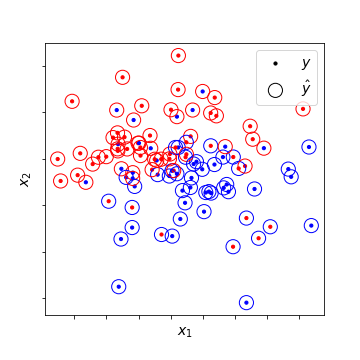
\includegraphics[width=\textwidth]{../plots_teoria/intro_scatterplot.png}
        \caption{Clasificación}
    \end{subfigure}
    \hfill
    \begin{subfigure}[t]{0.4\textwidth}
        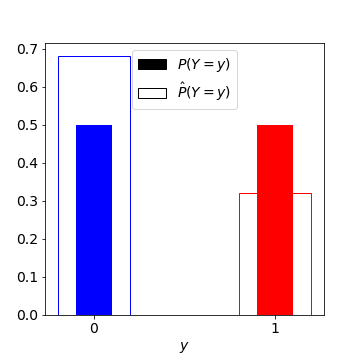
\includegraphics[width=\textwidth]{../plots_teoria/intro_barplot.png}
        \caption{Cuantificación}
    \end{subfigure}
    \caption{En la clasificación, la predicción es a nivel individual, mientras
    que en la cuantificación es a nivel agregado.}\label{fig:intro}
\end{figure}

En resumen, y generalizando no sólo para clasificación sino también a otros
problemas (regresión, ordinalidad, etc), la tarea de cuantificación consiste en
proporcionar predicciones agregadas para conjuntos de datos, en vez de
predicciones particulares sobre los datos individuales. Si bien en principio no
es necesario realizar predicciones por cada individuo, muchos de los métodos se
basan en obtener la cuantificación de esa manera, ya que hacer predicciones
individuales suele ser un requisito de por sí de las aplicaciones prácticas, o
porque ya existen en ellas modelos que las generen.

La literatura sobre métodos relacionados con cuantificación está un tanto
desconectada. Algunos de los métodos que pueden usarse como cuantificadores han
sido ideados para otros fines, principalmente para mejorar la precisión en
clasificación cuando cambia el dominio. El desempeño de este último grupo ha
sido normalmente estudiado solo en términos de mejora en las tareas de
clasificación pero no como cuantificadores. Dado este escenario, y debido a la
variedad de campos en los que ha surgido como una necesidad de aplicación, los
algoritmos que se pueden aplicar para tareas de cuantificación aparecen en
artículos que usan diferentes palabras clave y nombres, como {\it
counting\/}~\cite{lewis1995evaluating}, {\it prior probability
shift\/}~\cite{moreno2012unifying, storkey2009training}, {\it posterior
probability estimation\/}~\cite{alaiz2011class}, {\it class prior
estimation\/}~\cite{du2014class, chan2006estimating, zhang2010transfer}, {\it
class prior change\/}~\cite{du2014semi}, {\it prevalence
estimation\/}~\cite{barranquero2013study}, {\it class ratio
estimation\/}~\cite{asoh2012fast} o {\it class distribution
estimation\/}~\cite{gonzalez2013class, limsetto2011handling,
xue2009quantification}, por citar solo algunos de ellos.

\section{Tipos de Cuantificación}\label{problema:tipos}

Aunque el estudio de la cuantificación se ha centrado principalmente en el
dominio de clasificación, la cuantificación también aparece en otros tipos de
problemas de aprendizaje automático, como la regresión, la clasificación
ordinal, el aprendizaje sensible al costo y la cuantificación en redes.

De manera similar a la regresión, aprender a cuantificar admite diferentes
problemas de interés aplicativo, basados en cuántas clases distintas existen en
el problema, y en cuántas de las clases se pueden atribuir al mismo tiempo al
mismo individuo. Así, los problemas de cuantificación se dividen de esta manera:

\begin{enumerate}
    \item Etiquetado simple {\it (Single-Label Quantification -SLQ-)\/}: cuando
    cada individuo pertenece exactamente a una de las clases en
    $C=\{c_1,\dots,c_{\#C}\}$.
    \item Etiquetado múltiple {\it (Multi-Label Quantification -MLQ-)\/}: cuando
    cada individuo puede pertenecer a cualquier número de clases (cero, una o
    varias) en $C=\{c_1,\dots,c_{\#C}\}$.
    \item Cuantificación Binaria {\it (Binary Quantification -BQ-)\/}:
    \begin{enumerate}
        \item en {\it SLQ\/} con $\#C=2$, (en este caso $C=\{c_1,c_2\}$, y cada
        individuo pertenece a $c_1$ o $c_2$)
        \item en {\it MLQ\/} con $\#C=1$, (en este caso $C=\{c\}$, y cada
        individuo pertenece o no a $c$)
    \end{enumerate}
    \item Cuantificación Ordinal {\it (Ordinal Quantification -OQ-)\/}: cuando
    existe un orden $c_1 \prec \dots \prec c_{\#C}$ en
    $C=\{c_1,\dots,c_{\#C}\}$.
    \item Cuantificación de Regresión {\it (Regression Quantification -RQ-)\/}:
    cuando no hay un conjunto de clases involucradas, sino que cada individuo
    está etiquetado con una puntuación de valor real y la cuantificación
    equivale a estimar la fracción de ítems cuya puntuación está en un intervalo
    dado $[a, b]$ con ${a, b \in \mathbb{R}^d}$.
\end{enumerate}

\section{Marco teórico}\label{problema:marco_teorico}

Si hablamos entonces de cuantificación binaria, se tiene que por cada muestra $i
\in \{1,\dots,n\}$, $(\boldsymbol{X}_i,Y_i,S_i)$ es un vector de variables
aleatorias tal que $\boldsymbol{X}_i \in \mathbb{R}^d$ son las características
de la muestra, $Y_i \in C$ con $C=\{1,0\}$ indica la clase a la que pertenece y
$S_i \in \{1,0\}$ indica si fue etiquetada (y pertenece entonces al conjunto de
entrenamiento) o no. Es decir, cuando $S_i=0$, entonces $Y_i$ no es observable.
El objectivo es estimar $\theta:= \mathbb{P}(Y=1|S=0)$\footnote{En
cuantificación, se lo nombra generalmente como $p$ (o $p_1,\dots,p_{\#C}$ o
$p(c)$ para el caso multiclase) en vez de $\theta$, por lo que en este trabajo
también se usará esta nomenclatura.}, es decir, la prevalencia de etiquetas
positivas entre muestras no etiquetadas. Esta prevalencia no se asume de ser la
misma que en las muestras etiquetadas, $\mathbb{P}(Y=1|S=1)$. Además, el
estimador de $\theta$ debe depender sólo de los datos disponibles, es decir, de
las características de todas las muestras y de las etiquetas que fueron
obtenidas. Los supuestos que se asumen~\cite{vaz2019quantification} son:

\begin{itemize}
  \item $(\boldsymbol{X}_1,Y_1,S_1) \dots (\boldsymbol{X}_n,Y_n,S_n)$ son
  independientes
  \item Por cada $s \in \{0,1\}$,
  $(\boldsymbol{X}_1,Y_1)|S_1=s,\dots,(\boldsymbol{X}_n,Y_n)|S_n=s$ son
  idénticamente distribuidas.
  \item Por cada $(y_1,\dots,y_n)\in{\{0,1\}}^n$,
  $(\boldsymbol{X}_1,\dots,\boldsymbol{X}_n)$ es independiente de
  $(S_1,\dots,S_n)$ condicionado a $(Y_1,\dots,Y_n)=(y_1,\dots,y_n)$
\end{itemize}

Usando la distribución de probabilidad conjunta, podemos factorizar usando las
distribuciones condicionales:
\begin{equation}
    \mathbb{P}(\boldsymbol{X},Y,S)=\mathbb{P}(\boldsymbol{X}|Y,S)\mathbb{P}(Y|S)\mathbb{P}(S)
\end{equation}
Luego, usando el tercer supuesto mencionado, podemos
hacer~\cite{moreno2012unifying}:
\begin{equation}
    \mathbb{P}(\boldsymbol{X},Y,S)=\mathbb{P}(\boldsymbol{X}|Y)\mathbb{P}(Y|S)\mathbb{P}(S)
\end{equation}
Si bien existen varios métodos propuestos para el aprendizaje de
cuantificación~\cite{esuli2023learning, gonzalez2017review}, el mismo es todavía
relativamente desconocido incluso para expertos en aprendizaje automático. La
razón principal es la creencia errónea de que es una tarea trivial que se puede
resolver usando un método directo, como {\it CC}. La cuantificación requiere
métodos más sofisticados si el objetivo es obtener modelos óptimos, y su
principal dificultad radica en la definición del problema, ya que las
distribuciones de los datos de entrenamiento y de prueba pueden ser distintas.
Por ejemplo, si la diferencia entre $\mathbb{P}(Y=1|S=0)$ y
$\mathbb{P}(Y=1|S=1)$ es grande, los métodos simples como {\it CC\/} suelen
tener bajo rendimiento.


\section{Cambios en las distribuciones de los datos}\label{problema:cambios}

En lo últimos años ha habido un interés creciente en las aplicaciones que
presentan cambios en las distribuciones de datos (conocido en la blibliografía
por su término en inglés {\it dataset shift\/}). Estos problemas comparten el
hecho de que la distribución de los datos utilizados para entrenar es diferente
a la de los datos que se usan para predecir. Al igual que para el área de la
cuantificación, aquí también la literatura sobre el tema está dispersa y
diferentes autores usan diferentes nombres para referirse a los mismos
conceptos, o usan el mismo nombre para diferentes conceptos.

Teniendo en cuenta que en los problemas de clasificación tenemos:

\begin{itemize}
    \item Un conjunto de características o covariables $\boldsymbol{X}$.
    \item Una variable de respuesta $Y$.
    \item Una distribución de probabilidad conjunta
    $\mathbb{P}(Y=y,\boldsymbol{X=x})$.
\end{itemize}

La probabilidad conjunta $\mathbb{P}(Y,\boldsymbol{X})$ luego se puede escribir
como $\mathbb{P}(Y|\boldsymbol{X})\mathbb{P}(\boldsymbol{X})$ o como
$\mathbb{P}(\boldsymbol{X}|Y)\mathbb{P}(Y)$. Por otro lado, cuando usamos los
términos de entrenamiento ({\it train\/}) y prueba ({\it test\/}), nos referimos
a las datos disponibles para entrenar al clasificador y los datos presentes en
el entorno en el que se implementará el clasificador, respectivamente. Podemos
entonces también separar los datos en dos distribuciones distintas,
condicionando a la vaiable $S$ definida en~\ref{problema:marco_teorico}, siendo
$\mathbb{P}_{tr}(Y,\boldsymbol{X})=\mathbb{P}(Y,\boldsymbol{X}|S=1)$ y
$\mathbb{P}_{tst}(Y,\boldsymbol{X})=\mathbb{P}(Y,\boldsymbol{X}|S=0)$.

El {\it dataset shift\/} aparece cuando las distribuciones conjuntas de
entrenamiento y de prueba son diferentes, es decir, cuando
$\mathbb{P}_{tr}(Y,\boldsymbol{X}) \neq
\mathbb{P}_{tst}(Y,\boldsymbol{X})$.~\citet{moreno2012unifying} distingue las
distintas variantes del {\it dataset shift\/} según qué elementos mencionados
anteriormente cambian:

\begin{itemize}
    \item {\it Covariate shift}, cuando $\mathbb{P}_{tr}(Y|\boldsymbol{X}) =
    \mathbb{P}_{tst}(Y|\boldsymbol{X})$ y $\mathbb{P}_{tr}(\boldsymbol{X}) \neq
    \mathbb{P}_{tst}(\boldsymbol{X})$
    \item {\it Prior probability shift}, cuando
    $\mathbb{P}_{tr}(\boldsymbol{X}|Y) = \mathbb{P}_{tst}(\boldsymbol{X}|Y)$ y
    $\mathbb{P}_{tr}(Y) \neq \mathbb{P}_{tst}(Y)$
    \item {\it Concept shift}, cuando $\mathbb{P}_{tr}(Y|\boldsymbol{X}) \neq
    \mathbb{P}_{tst}(Y|\boldsymbol{X})$ y $\mathbb{P}_{tr}(\boldsymbol{X}) =
    \mathbb{P}_{tst}(\boldsymbol{X})$ o $\mathbb{P}_{tr}(\boldsymbol{X}|Y) \neq
    \mathbb{P}_{tst}(\boldsymbol{X}|Y)$ y $\mathbb{P}_{tr}(Y) =
    \mathbb{P}_{tst}(Y)$
\end{itemize}

Otros tipos de {\it dataset shift\/} surgen cuando
$\mathbb{P}_{tr}(Y|\boldsymbol{X}) \neq \mathbb{P}_{tst}(Y|\boldsymbol{X})$ y
$\mathbb{P}_{tr}(\boldsymbol{X}) \neq \mathbb{P}_{tst}(\boldsymbol{X})$ y cuando
$\mathbb{P}_{tr}(\boldsymbol{X}|Y) \neq \mathbb{P}_{tst}(\boldsymbol{X}|Y)$ y
$\mathbb{P}_{tr}(Y) \neq \mathbb{P}_{tst}(Y)$. Sin embargo, estos tipos de
cambios no se consideran generalmente en la literatura ya que aparecen mucho más
raramente, o incluso porque son dificiles o imposibles de resolver.

El problema de cuantificación se trata de un caso donde $\mathbb{P}_{tst}(Y)$ es
desconocido. Además, la mayoría de los métodos de cuantificación propuestos
asumen que $\mathbb{P}_{tr}(\boldsymbol{X}|Y) =
\mathbb{P}_{tst}(\boldsymbol{X}|Y)$, por lo que están dentro de los casos de
{\it prior probability shift}.

Por otro lado, en la mayoría de los casos el objetivo final de la implementación
es estimar algún parámetro de $\mathbb{P}_{tst}(Y)$. Por ejemplo, como ya
mencionamos anteriormente, en la cuantificación binaria, se desea estimar
$\theta:= \mathbb{P}(Y=1|S=0)$, o lo que es lo mismo, $p_{tst}:=
\mathbb{P}_{tst}(Y=1)$. Es decir, en la cuantificación la tarea indirectamente
suele ser aprender a aproximar una distribución desconocida (observando sólo
características de una muestra) mediante una distribución conocida. En
consecuencia, prácticamente todas las medidas de evaluación para la
cuantificación son divergencias, es decir, medidas de cómo una distribución
pronosticada difiere de la distribución real.

\begin{figure}[h]
    \centering
    \begin{subfigure}[t]{0.4\textwidth}
        \centering
        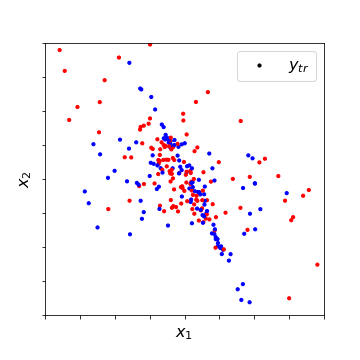
\includegraphics[width=\textwidth]{../plots_teoria/cambios_train_scatterplot.png}
        \caption{Muestra de entrenamiento}\label{cambios:datos_tr}
    \end{subfigure}
    \hfill
    \begin{subfigure}[t]{0.4\textwidth}
        \centering
        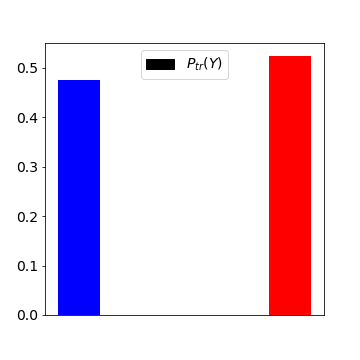
\includegraphics[width=\textwidth]{../plots_teoria/cambios_train_barplot.png}
        \caption{Prevalencia de clases en muestra de
        entrenamiento}\label{cambios:prevalencia_tr}
    \end{subfigure}
    \medskip
    \begin{subfigure}[t]{0.4\textwidth}
        \centering
        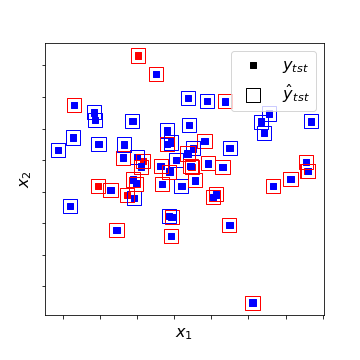
\includegraphics[width=\textwidth]{../plots_teoria/cambios_test_scatterplot.png}
        \caption{Clasificación en muestra de prueba. Para el modelo, las
        $y_{tst}$ son desconocidas.}\label{cambios:clasificacion_tst}
    \end{subfigure}
    \hfill
    \begin{subfigure}[t]{0.4\textwidth}
        \centering
        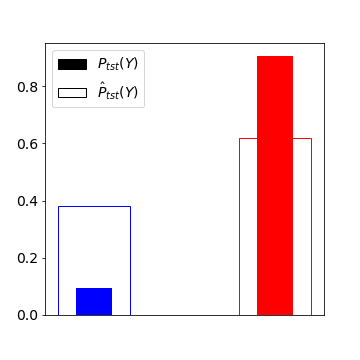
\includegraphics[width=\textwidth]{../plots_teoria/cambios_test_barplot.png}
        \caption{Prevalencia de clases verdadera y cuantificación en muestra de
        prueba}\label{cambios:cuantificacion_tst}
    \end{subfigure}
    \caption{El {\it prior probability shift\/} propio de los problemas de
    cuantificación puede hacer que los métodos simples de cuantificación, como
    {\it CC}, tengan grandes errores.}\label{fig:cambios}
\end{figure}

\section{El problema de clasificar y contar}\label{problema:clasificar_y_contar}

En ausencia de métodos para estimar los valores de prevalencia de clase de forma
directa, el primer método que suele pensarse para hacerlo es {\it Classify \&
Count}, es decir, clasificar cada individuo sin etiquetar y estimar los valores
de prevalencia de clase contando los individuos que fueron asignados a cada
clase. Sin embargo, esta estrategia es subóptima: si bien un clasificador
perfecto es también un cuantificador perfecto, un buen clasificador puede ser un
mal cuantificador. Para ver esto, se puede ver la definición de $F_1$, una
función de evaluación estándar para la clasificación binaria, que se define
como:
\begin{equation}
    F_1 = \frac{2 \cdot tp}{2 \cdot tp + fp + fn}
\end{equation}
donde $tp$, $fp$, $fn$ indican el número de verdaderos positivos, falsos
positivos y falsos negativos, respectivamente. Un buen clasificador puede ser un
mal cuantificador ya que $F_1$ considera buenos aquellos clasificadores que
mantienen la suma $fp + fn$ al mínimo; sin embargo, el objetivo de un algoritmo
de cuantificación debe ser mantener al mínimo $|fp-fn|$.

El análisis teórico de esta cuestión se basa en el supuesto de {\it prior
probability shift\/}~\ref{problema:cambios}. Bajo tal supuesto, la estimación
$\hat p$ obtenida por el enfoque {\it CC\/} depende sólo de las características
del clasificador, definido (para el caso binario) por su tasa de verdaderos
positivos ($tpr$), su tasa de falsos positivos ($fpr$) y de la prevalencia real
($p$):
\begin{equation}\label{ecuacion:tpr_fpr}
    \hat p(p) = p \cdot {tpr} + (1-p) \cdot {fpr}
\end{equation}
\begin{figure}[h]
    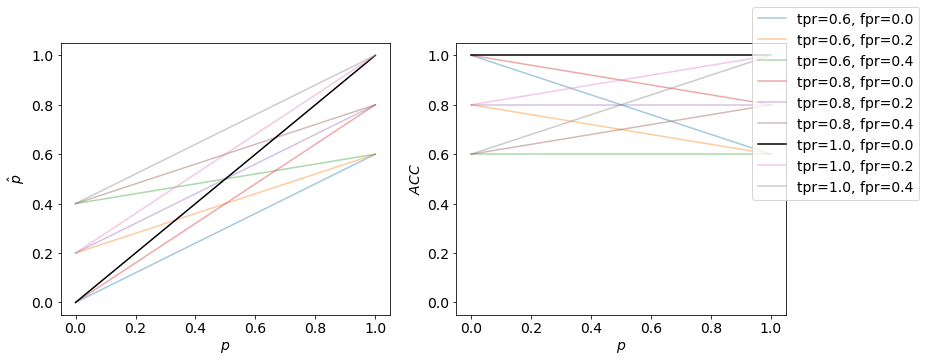
\includegraphics[width=\textwidth]{../plots_teoria/cc_tpr_fpr.png}
    \caption{La línea negra representa el cuantificador y clasificador perfecto,
    respectivamente. Las otras líneas muestran las estimaciones teóricas de
    $\hat p$ resultantes de aplicar la ecuación~\ref{ecuacion:tpr_fpr}, y el
    {\it accuracy\/} correspondiente al clasificador, según se varían los
    valores de $tpr$ y $fpr$}\label{fig:cc_tpr_fpr}
\end{figure}

El mal desempeño de {\it CC\/} fue demostrado mediante el siguiente teorema
por~\citet{forman2008quantifying}:

\begin{theorem}[Toerema de Forman]
    \citep[p.169]{forman2008quantifying}\label{teorema:forman} Para un
    clasificador imperfecto, el método {\it CC\/} subestimará la porporción
    verdadera de ejemplos positivos $p$ en un conjunto de prueba para $p>p^*$, y
    sobreestimará para $p<p^*$, donde $p^*$ es la proporción particular en la
    cual el método {\it CC\/} estima de forma correcta. Es decir, el método {\it
    CC\/} estima exactamente $p^*$ para un conjunto de prueba con $p^*$ muestras
    positivas.
\end{theorem}

La demostración (ver todos los detalles en~\citep[p.170]{forman2008quantifying})
supone que el cuantificador {\it CC\/} produce una predicción perfecta para una
prevalencia concreta, llamada $p^*$, y estudia su comportamiento cuando la
prevalencia cambia ligeramente. Suponiendo que $\hat p(p^*) = p^*$, cuando la
prevalencia cambia en una cantidad $\Delta \neq 0, p^* + \Delta$, la estimación
del método CC en tal caso será:
\begin{align}
\begin{split}
    \hat p(p^* + \Delta) &= (p^* + \Delta) \cdot {tpr} + (1-(p^* + \Delta)) \cdot {fpr} \\
    &= \hat p(p^*) + ({tpr} - {fpr}) \cdot \Delta \\
    &= p^* + ({tpr} - {fpr}) \cdot \Delta
\end{split}
\end{align}
La predicción del método {\it CC\/} será perfecta, $\hat p(p^* + \Delta) = (p^*
+ \Delta)$, sólo cuando el clasificador también es perfecto (${tpr} = 1$, ${fpr}
= 0$ y por tanto ${tpr} - {fpr} = 1$). Pero en el caso habitual, en el cual el
clasificador es imperfecto ($0 \leq {tpr} - \text {fpr} < 1$), cuando la
prevalencia aumenta ($\Delta > 0$), {\it CC\/} la subestima ($\hat p < p^* +
\Delta $), y cuando la prevalencia disminuye ($\Delta < 0$), {\it CC\/} la
sobreestima ($\hat p > p^* + \Delta $).

Un buen clasificador puede estar sesgado, es decir, puede mantener sus falsos
positivos al mínimo sólo a expensas de una cantidad sustancialmente mayor de
falsos negativos (o viceversa); si este es el caso, el clasificador es un mal
cuantificador. Este fenómeno no es infrecuente, especialmente en presencia de
datos desbalanceados. En tales casos, los algoritmos que minimizan las funciones
de pérdida de clasificacion ({\it Hamming}, {\it hinge}, etc) suelen generar
clasificadores con tendencia a elegir la clase mayoritaria, lo que implica un
número mucho mayor de falsos positivos que de falsos negativos para la clase
mayoritaria, lo que significa a su vez que tal algoritmo tenderá a subestimar
las clases minoritarias.

Los argumentos anteriores indican que no se debe considerar la cuantificación
como un mero subproducto de la clasificación, y debe estudiarse y resolverse
como una tarea en sí misma. Hay al menos otros dos argumentos que apoyan esta
idea. Uno es que las funciones que se utilizan para evaluar la clasificación no
se pueden utilizar para evaluar la cuantificación, ya que estas funciones miden,
en general, cuántos individuos han sido mal clasificados, y no cuánto difiere la
prevalencia de clase estimada del valor real. Esto significa que los algoritmos
que minimizan estas funciones están optimizados para la clasificación, y no para
la cuantificación. Un segundo argumento presentado por
~\citet{forman2008quantifying} es que los métodos diseñados específicamente para
cuantificar requieren menos datos de entrenamiento para alcanzar la misma
precisión de cuantificación que los métodos estándar basados en {\it CC}. Si
bien esta observación es de naturaleza empírica, también existen argumentos
teóricos que sustentan este hecho~\cite{vapnik1999overview}.

\section{Cuantificadores para la mejora de la
clasificación}\label{problema:mejora}

Debido a los problemas mencionados anteriormente de los clasificadores frente a
cambios en las distribuciones de los datos y frente a datos desbalanceados, los
algoritmos de cuantificación están cada vez más frecuentemente también siendo
usados en tareas que requieren predicciones individuales. Los mismos se emplean
como suplemento de clasificadores para suplir sus defectos frente a estos
problemas, ya que en algunos casos no sólo predicen los valores agregados, sino
que también mejoran las predicciones a nivel individual.

Por ejemplo, el {\it prior probability shift\/} puede hacer que los
clasificadores performen de manera subóptima. En el caso del clasificador óptimo
de Bayes, dado por:
\begin{equation}\label{ecuacion:bayes}
    h(\boldsymbol{x}) = \argmax_{y} p_{Y|\boldsymbol{X}=\boldsymbol{x}}(y) = \argmax_{y} \frac{p_{\boldsymbol{X}|Y=y}(\boldsymbol{x})p_Y(y)}{p_{\boldsymbol{X}}(\boldsymbol{x})}
\end{equation}
la decisión del clasificador depende de $p_Y(y)$, que es estimado con el dataset
de entrenamiento, siendo $\hat p_Y(y=1) = p_{tr}$. Es decir, que en caso de
$\mathbb{P}_{tr}(Y) \neq \mathbb{P}_{tst}(Y)$, la decisión final del
clasificador puede verse afectada negativamente. Para mejorar el rendimiento del
clasificador frente a estos casos, se debería usar $\hat p_Y(y=1) = p_{tst}$,
pero como $p_{tst}$ es generalmente desconocido, se puede usar un método de
cuantificación para estimarlo~\cite{saerens2002adjusting, alaiz2011class,
zhang2010transfer, xue2009quantification}.

\begin{figure}[H]
    \centerline{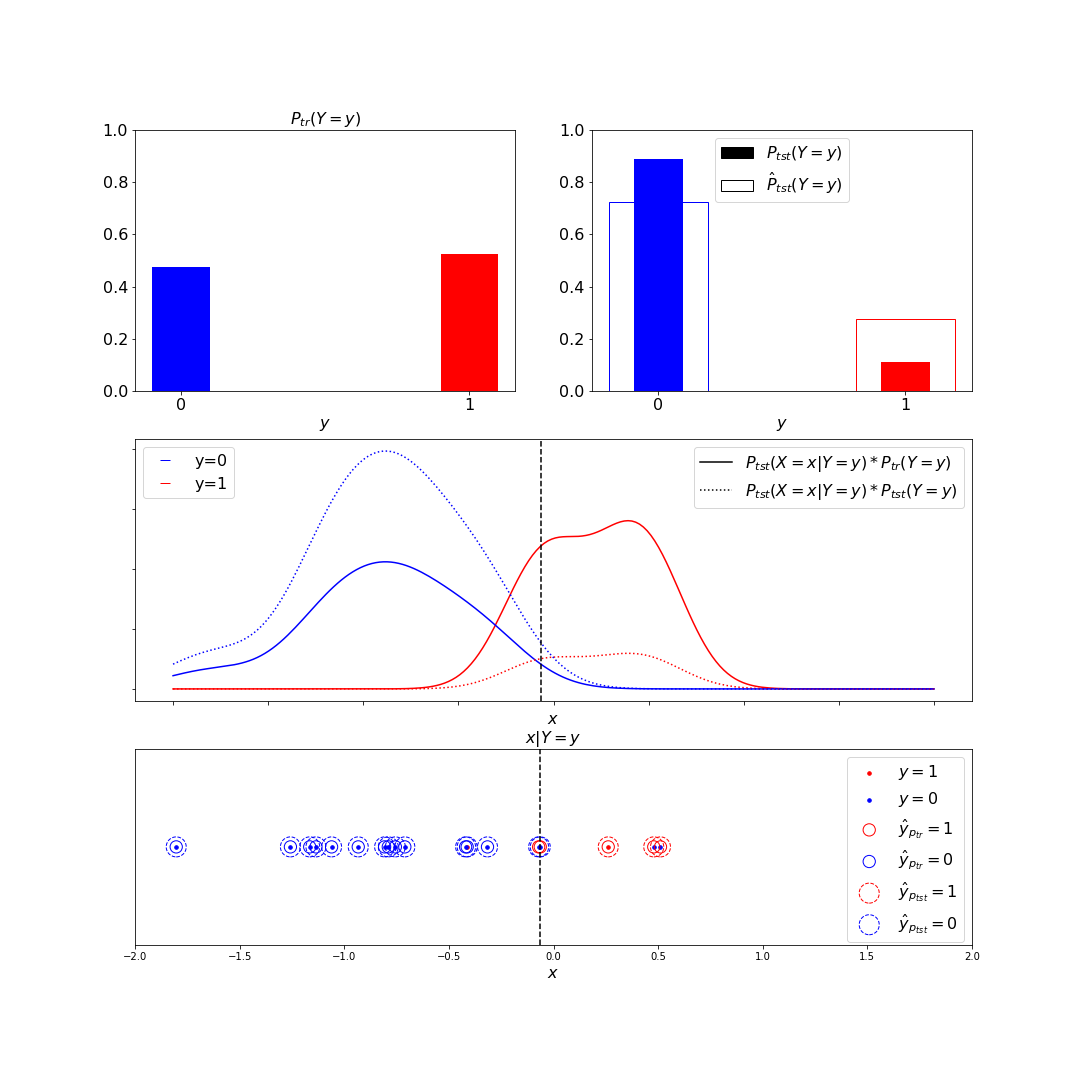
\includegraphics[width=0.75\textwidth]{../plots_teoria/bayes_classifier.png}}
    \caption{Ejemplo de como el {\it prior probability shift\/} puede alterar
    las predicciones del clasificador óptimo de Bayes. Vemos que si usaramos
    $\mathbb{P}_{tst}(Y)$ en vez de $\mathbb{P}_{tr}(Y)$, en este caso pasaría a
    predecir la clase azúl en vez de roja para toda
    $\boldsymbol{x}$.}\label{fig:bayes_classifier}
\end{figure}

Los métodos de cuantificación pueden usarse no sólo para mejorar el rendimiento
general de un clasificador, sino también para mejorar su equidad o {\it
fairness\/}~\cite{biswas2021ensuring}, es decir, su posibilidad de predecir
resultados independientes de un cierto conjunto de variables que consideramos
sensibles y no relacionadas con él (e.j.:~género, etnia, orientación sexual,
etc.). Por ejemplo, suponiendo que una variable $S$ debe considerarse sensible,
se puede estimar $\mathbb{P}_{tr}(Y|S)$. Luego, si los datos de entrenamiento
están sesgados, por ejemplo, con $\mathbb{P}_{tr}(Y=1|S=1) \gg
\mathbb{P}_{tr}(Y=1|S=0)$, pero se sabe que en las muestras a inferir esto no es
así, se puede optimizar el modelo de clasificación imponiento alguna penalidad
basada en la estimación de $\mathbb{P}_{tst}(Y|S)$, siendo esta última obtenido
por un cuantificador.

\chapter{Métodos de Estimación}\label{estimacion}

Durante los últimos años, se han propuesto varios métodos de cuantificación
desde diferentes perspectivas y con diferentes objetivos. En términos generales,
se pueden distinguir dos grandes clases de métodos en la literatura. La primera
clase es la de métodos agregativos, es decir, métodos que requieren la
clasificación de todos los individuos como un paso intermedio. Dentro de los
métodos agregativos, se pueden identificar dos subclases. La primera subclase
incluye métodos basados en clasificadores de propósito general; en estos métodos
la clasificación de los elementos individuales realizados como un paso
intermedio puede lograrse mediante cualquier clasificador. La segunda subclase
se compone, en cambio, de métodos que para clasificar los individuos, se basan
en métodos de aprendizaje diseñados con la cuantificación en mente. La segunda
clase es la de métodos no agregativos, es decir, métodos que resuelven la tarea
de cuantificación “holísticamente”, es decir, sin clasificar a los individuos.
La idea de esta tesis no es la de mostrar todos los métodos propuestos hasta la
actualidad, sino la de mencionar los métodos más populares.

\subsubsection{Caso de Ejemplo}\label{estimacion:ejemplo}

Como ejemplo de muestra para comparar los distintos métodos de estimación, se
usará el mismo set de datos artificiales que en las figuras~\ref{fig:intro}
y~\ref{fig:cambios}. Para crear el set de datos se utilizó el algoritmo
prepuesto por~\citet{Guyon2003DesignOE} mediante la
función~\href{https://scikit-learn.org/stable/modules/generated/sklearn.datasets.make_classification.html}{{\it
make\_classification}} de {\it scikit-learn}, usando los siguientes parámetros
de entrada:

\begin{python}
population_size = 150 X, y = make_classification( n_samples=population_size,
n_features=2, n_informative=2, n_redundant=0, n_repeated=0,
n_clusters_per_class=2, n_classes=2, weights=None, class_sep=0.1,
random_state=42, )
\end{python}

Esta función, al usar \(weights=None\), crea un set de datos balanceados en
cuanto a las clases de los individuos (figura~\ref{fig:intro}). Sin embargo,
para poder evaluar los distintos métodos, lo que haremos ahora es seleccionar
100 individuos y usarlos como datos de entrenamiento, y hacer un sub-muestreo de
los 50 restantes de forma tal de aproximarnos a un \(p_{tst}=0.1\):

\begin{python}
train_size = 100 prev_test = 0.1 X_train, y_train = X[:train_size],
y[:train_size] X_test, y_test = X[train_size:], y[train_size:]
idx_negatives_test = np.argwhere(y_test==0).flatten() idx_positives_test =
np.random.choice( np.argwhere(y_test==1).flatten(),
size=round((prev_test)*len(idx_negatives_test)/(1-prev_test)), replace=False )
idx_test = np.concatenate([idx_positives_test, idx_negatives_test]) X_test =
X_test[idx_test] y_test = y_test[idx_test]
\end{python}

El código de arriba termina generando un set de entrenamiento de tamaño
\(n_{tr}=100\) con \(p_{tr}=0.53\) (figuras~\ref{cambios:datos_tr}
y~\ref{cambios:prevalencia_tr}) y uno de prueba de tamaño \(n_{tst}=31\) con
\(p_{tst}\approx0.097\) (figuras~\ref{cambios:clasificacion_tst}
y~\ref{cambios:cuantificacion_tst}).

El modelo de clasificación utilizado para generar las predicciones mostradas en
ambas figuras~\ref{fig:intro} (entrenando y prediciendo con todos los datos)
y~\ref{fig:cambios} (entrenando con los datos de entrenamiento y prediciendo los
de prueba) es el clasificador {\it Naive Bayes\/} generado mediante la
clase~\href{https://scikit-learn.org/stable/modules/generated/sklearn.naive_bayes.GaussianNB.html}{{\it
GaussianNB}} de {\it scikit-learn}, usando sus parámetros por default.

\section{Métodos Agregativos}\label{estimacion:agregativos}

\subsection{Con clasificadores generales}\label{estimacion:generales}

Dentro de los métodos agregativos, algunos de ellos requieren como entrada las
etiquetas de clases predichas (es decir, el tipo de salida que devuelven los
clasificadores denominados duros), otros requieren un {\it score\/} de decisión
(como podría ser la distancia al hiperplano de separación en el clasificador
SVM), y otros que requieren como entrada las probabilidades {\it a posteriori\/}
de pertenencia a cada clase (es decir, el tipo de salida que devuelven los
clasificadores denominados blandos)\footnote{Los clasificadores blandos y de
{\it score\/} se pueden convertir en duros usando umbrales de clasificación}. En
estos últimos, además, las probabilidades {\it a posteriori\/} deben estar
calibradas (para mayor información sobre calibración consultar el
Apéndice~\ref{appendix:calibracion}). Para estos casos, en los ejemplos a
continuación que requieren clasificadores blandos se separó de las muestras de
entrenamiento un 15\% de datos para el proceso de calibración (y estratificando
para que la proporción de etiquetas se mantenga igual).

\subsubsection{Clasificar y Contar (CC)}\label{estimacion:cc}

El método más sencillo y directo para construir un cuantificador para
clasificación (tanto binaria como multiclase) es aplicar el enfoque {\it
Classify \& Count\/}~\cite{forman2005counting}. {\it CC\/} juega un papel
importante en la investigación de cuantificación ya que siempre se utiliza como
el {\it baseline\/} que cualquier método de cuantificación razonable debe
mejorar. Este método consiste simplemente en: (i) ajustar un clasificador duro,
y luego (ii), utilizando dicho clasificador, clasificar las instancias de la
muestra de prueba, contando la proporción de cada clase. Generalizando el
estimador de {\it CC\/} para el caso multiclase, el mismo queda entonces
definido por:
\begin{equation}
    \hat p^{\it CC\/}_{tst}(c) = \frac{\#\{\boldsymbol{x} \in \boldsymbol{X}_{tst}|h_{tr}(\boldsymbol{x})=c\}}{\#\boldsymbol{X}_{tst}}\label{ecuacion:cc}
\end{equation}
donde se usó \(h_{tr}\) para la función de decisión del clasificador duro
ajustado con la muestra de entrenamiento.

Es evidente que podemos obtener un cuantificador perfecto si el clasificador es
también perfecto. El problema es que obtener un clasificador perfecto es casi
imposible en aplicaciones reales, y luego el cuantificador hereda el sesgo del
clasificador. Este aspecto se analiza en varios artículos tanto desde una
perspectiva teórica como práctica, como lo hizo~\citet{forman2008quantifying}, y
como también ya lo hemos mencionado en~\ref{problema:clasificar_y_contar}.

\paragraph{\it Ejemplo:\/} Para el caso de ejemplo, y manteniendo el
clasificador allí usado, debemos contar la cantidad de predicciones positivas
(rojas) en la figura~\ref{fig:cambios}, y dividirlas por el tamaño de la muestra
de prueba. Es decir, \(\hat p^{\it CC\/}_{tst}(c=1) = \frac{23}{31} \approx
0.742\).

\subsubsection{Clasificar, Contar y Ajustar (ACC)}\label{estimacion:acc}

Conocido en inglés como {\it Adjusted Classify \& Count}, {\it Adjusted
Count\/}~\cite{forman2008quantifying} o también como {\it Confusion Matrix
Method\/}~\cite{saerens2002adjusting}, este método se basa en corregir las
estimaciones de {\it CC\/} teniendo en cuenta la tendencia del clasificador a
cometer errores de cierto tipo. Un modelo {\it ACC\/} está compuesto por dos
elementos: un clasificador duro (como en {\it CC\/}) y de las estimaciones de
\(tpr\) y \(fpr\). Dichas estimaciones pueden obtenerse usando validación
cruzada o {\it cross-validation}, ya sea mediante la técnica de {\it k-folds\/}
o un {\it held-out}. Luego, en la fase de predicción, el modelo obtiene una
primera estimación \(\hat p\) de la misma forma que en {\it CC\/} que luego,
para el caso binario, es ajustado aplicando la siguiente fórmula\footnote{A
veces, esta expresión conduce a un valor inválido de \(\hat p^{\it
ACC\/}_{tst}\) que debe recortarse en el rango \([0, 1]\) en un último paso.}:
\begin{equation}
    \hat p^{\it ACC\/}_{tst}(c=1) = \frac{\hat p^{\it CC\/}_{tst}(c=1)-\hat{fpr}}{\hat{tpr} - \hat{fpr}}\label{ecuacion:acc_binaria}
\end{equation}
Esta expresión se obtiene despejando la verdadera prevalencia \(p\) de la
ecuación~\ref{ecuacion:tpr_fpr} y reemplazando \(fpr\) y \(tpr\) por sus
estimadores.

El método {\it ACC\/} es teóricamente perfecto, independientemente del valor de
{\it accuracy\/} obtenido con el clasificador, cuando se cumple el supuesto de
{\it prior probability shift\/}~\ref{problema:cambios} y cuando las estimaciones
de \(tpr\) y \(fpr\) son perfectas. Desafortunadamente, es raro que se cumplan
ambas condiciones en aplicaciones del mundo real:
\(\mathbb{P}(\boldsymbol{X}|Y)\) puede tener variaciones entre los datos de
entrenamiento y los de predicción, y es difícil obtener estimaciones perfectas
para \(tpr\) y \(fpr\) en algunos dominios ya que suelen haber pequeñas muestras
disponibles y/o están muy desequilibradas. Pero incluso en estos casos, el
rendimiento del método {\it ACC\/} suele ser mejor que el de {\it CC}.

Partiendo de la ecuación~\ref{ecuacion:cc} y utilizando el teorema de
probabilidad total, podemos extender la ecuación~\ref{ecuacion:acc_binaria} para
el caso multiclase:
\begin{align}
\begin{split}
    \hat p^{\it CC\/}_{tst}(c=c_k) &= \mathbb{\hat P}_{tst}(h_{tr}(\boldsymbol{x})=c_k) \\
    &= \sum \limits_{j=1}^{\#C}{\mathbb{\hat P}(h_{tr}(\boldsymbol{x})=c_k|y=c_j) \hat p^{\it ACC\/}_{tst}(c=c_j)}\label{ecuacion:acc_multiclase}
\end{split}
\end{align}
donde \(\hat p^{\it CC\/}_{tst}(c=c_k)\) es la fracción de datos de \(tst\) que
el clasificador \(h\) asigna a \(c_k\) (y por ende, es conocido), y
\(\mathbb{\hat{P}}(h_{tr}(\boldsymbol{x})=c_k|y=c_j)\) es la estimación de
probabilidad de que el clasificador \(h\) asigne la clase \(c_k\) a
\(\boldsymbol{x}\) cuando este pertenece a la clase \(c_j\). Estas
probabilidades, al igual que \(tpr\) y \(fpr\) en el caso binario, deben
estimarse mediante validación cruzada~\cite{barranquero2013study,
forman2005counting, forman2008quantifying}. Luego, \(\hat p^{\it
ACC\/}_{tst}(c=c_j)\), nuestras incógnitas (una por cada \(c_j\)), pueden
calcularse mediante un sistema de ecuaciones lineales con \(\#C\) ecuaciones y
\(\#C\) incógnitas.

\paragraph{\it Ejemplo:\/} Aquí debemos estimar el \(tpr\) y \(fpr\). Para ello,
se separó de la muestra de entrenamiento un 15\% de datos. Con el 85\% de la
muestra se entrenó el clasificador y se obtuvo un \(\hat p^{\it CC\/}_{tst}(c=1)
\approx 0.71\), y con el 15\% separado se obtuvo \(\hat{tpr} \approx 0.625\) y
\(\hat{fpr} \approx 0.714\), y por lo tanto, \(\hat p^{\it ACC\/}_{tst}(c=1)
\approx 0.0516\).

\subsubsection{Clasificar y Contar Probabilístico (PCC)}\label{estimacion:pcc}

Este método, conocido en inglés como {\it Probabilistic Classify and
Count\/}~\cite{bella2010quantification, tang2010network}, es una variante de
{\it CC\/} que utiliza un clasificador blando en vez de uno duro. Es decir, que
la salida del clasificador blando ajustado con la muestra de entrenamiento,
\(s(\boldsymbol{x}, y)\), será una estimación de la probabilidad {\it a
posteriori\/} \({p}_{Y|\boldsymbol{X}=\boldsymbol{x}}(y)\) por cada individuo
\(\boldsymbol{x} \in \boldsymbol{X}_{tst}\) y cada \(y \in C\). El método
consiste en estimar las \({p}_{tst}(c=c_j)\) mediante el valor esperado de la
proporción de items que se predijeron como pertenecientes a cada clase \(c_j\):
\begin{align}
\begin{split}
    \hat p^{\it PCC\/}_{tst}(c=c_j) &= \mathbb{\hat E}[p_{Y|\boldsymbol{X}=\boldsymbol{x}}(y=c_j)] \\
    &= \frac{1}{m} \sum \limits_{i=1}^{m}{\hat p_{Y|\boldsymbol{X}=\boldsymbol{x}_i}(y=c_j)} \\
    &= \frac{1}{m} \sum \limits_{i=1}^{m}{s(\boldsymbol{x}_i, y=c_j)}
\end{split}
\end{align}
con \(m=\#\boldsymbol{X}_{tst}\). La intuición detrás de {\it PCC\/} es que las
probabilidades {\it a posteriori\/} contienen mayor información que las
decisiones de un clasificador duro y, por lo tanto, deberían ser usadas en su
lugar. Sin embargo,~\citet[Corolario 6, p.157 y p.163]{tasche2014exact}
demuestra que el comportamiento de {\it PCC\/} será similar al de {\it CC}, en
cuanto a que ambos subestiman o sobreestiman la prevalencia verdadera cuando la
distribución de clases cambia entre los datos de entrenamiento y de prueba.

\paragraph{\it Ejemplo:\/} Como este método utiliza un clasificador blando, se
separó primero un 15\% de los datos de entrenamiento. Con el 85\% se entrenó el
clasificador, y luego con el 15\% se realizó la calibración. Luego, debemos
sumar las salidas del clasificador calibrado para la clase positiva. Para el
ejemplo, se obtuvieron las siguientes salidas:
\begin{center}
    \begin{tabular}{lrrrrrrrrrrrrrrrrrrrrr}
        \toprule
        \textbf{$s(\boldsymbol{x}_i, y=1)$} & 0.54 & 0.54 & 0.49 & 0.50 & 0.45 &
        0.56 & 0.57 & 0.60 & 0.52 & 0.50 & 0.58 & 0.54 \ldots & 0.49 \\
        \bottomrule
    \end{tabular}
\end{center}
siendo \(\hat p^{\it PCC\/}_{tst}(c=1) \approx 0.527\).

\subsubsection{Clasificar, Contar y Ajustar Probabilístico
(PACC)}\label{estimacion:pacc}

Presentado como {\it Probabilistic Adjusted Classify and Count\/} o también como
{\it Probabilistic Adjusted Count}, este método combina las ideas de {\it ACC\/}
y de {\it PCC\/}~\cite{bella2010quantification, tang2010network}.
\begin{align}
\begin{split}
    \hat p^{\it PCC\/}_{tst}(c=c_k) &= \mathbb{\hat E}[\mathbb{P}_{tst}(h_{tr}(\boldsymbol{x})=c_k)] \\
    &= \mathbb{\hat E}[\sum \limits_{j=1}^{\#C}{\mathbb{P}(h_{tr}(\boldsymbol{x})=c_k|y=c_j) p^{\it PACC\/}_{tst}(c=c_j)}] \\
    &= \sum \limits_{j=1}^{\#C}\mathbb{\hat E}[{\mathbb{P}(h_{tr}(\boldsymbol{x})=c_k|y=c_j) p^{\it PACC\/}_{tst}(c=c_j)}] \\
    &= \sum \limits_{j=1}^{\#C}\mathbb{\hat E}[{\mathbb{P}(h_{tr}(\boldsymbol{x})=c_k|y=c_j)}] \hat p^{\it PACC\/}_{tst}(c=c_j) \\
    &= \sum \limits_{j=1}^{\#C} [\frac {1}{\#U_j} \sum_{\boldsymbol{x} \in U_j} \mathbb{\hat P}(h_{tr}(\boldsymbol{x})=c_k)] \hat p^{\it PACC\/}_{tst}(c=c_j)
\end{split}
\end{align}
donde \(U_j=\{(\boldsymbol{x}, y) \in (\boldsymbol{X}_{tst}, Y_{tst}) |
y=c_j\}\). Luego, \(\hat p^{\it PCC\/}_{tst}(c=c_k)\) se calcula mediante {\it
PCC\/} y, como en {\it ACC}, las \([\frac {1}{\#U_j} \sum_{\boldsymbol{x} \in
U_j} \mathbb{\hat{P}}(h_{tr}(\boldsymbol{x})=c_k)]\) deben estimarse mediante
validación cruzada, quedando nuevamente un sistema de ecuaciones lineales de
\(\#C\) ecuaciones y \(\#C\) incógnitas.

Para el caso particular binario, y relacionando con la
ecuación~\ref{ecuacion:acc_binaria}, tenemos:
\begin{equation}
    \hat p^{\it PACC\/}_{tst}(c=1) = \frac{\hat p^{\it PCC\/}_{tst}(c=1)-\hat{fp_{pa}}}{\hat{tp_{pa}}-\hat{fp_{pa}}}
\end{equation}

donde \(tp_{pa}\) y \(fp_{pa}\) ($pa$: {\it probability average\/}) son los dos
parámetros propios del cuantificador a estimar mediante validación cruzada,
siendo \(tp_{pa}\) el promedio de las probabilidades {\it a posteriori\/} para
la clase positiva estimadas por el clasificador correspondientes a los
individuos cuya etiqueta es positiva, y del mismo modo \(fp_{pa}\) pero para
individuos con etiqueta negativa. En este método hay que tener en cuenta ambas
consideraciones sobre las estimaciones de \(\hat p\) dentro del rango \([0, 1]\)
y sobre la calibración -ver~\ref{appendix:calibracion}-.

\paragraph{\it Ejemplo:\/} Del mismo modo que para el ejemplo de {\it PCC}, se
separó de la muestra de entrenamiento un 15\% de datos para realizar la
calibración del clasificador blando. Pero también se separó otro 15\% para
realizar el ajuste del propio método de cuantificación. Con el 70\% de datos se
entrenó el clasificador que luego fue calibrado usando el primer 15\% separado,
obteniendo un \(\hat p^{\it PCC\/}_{tst}(c=1) \approx 0.51\). Luego, con el
segundo 15\% de datos, se procedió a estimar \(tp_{pa}\) y \(fp_{pa}\). Teniendo
en cuenta entonces ahora tanto las salidas del clasificador calibrado como las
etiquetas de la muestra, tenemos:
\begin{center}
    \begin{tabular}{ccc}
        \toprule
        \(s(\boldsymbol{x}_i, y=0)\) &  \(s(\boldsymbol{x}_i, y=1)\) & \(c\) \\
        \midrule
        0.23 &    0.77 &  1 \\
        0.78 &    0.22 &  0 \\
        0.40 &    0.60 &  1 \\
        0.43 &    0.57 &  1 \\
        0.32 &    0.68 &  1 \\
        \ldots              \\
        0.58 &    0.42 &  0 \\
     \bottomrule
        \bottomrule
        \end{tabular}
\end{center}

siendo entonces \(\hat{tp_{pa}} \approx 0.551\) y \(\hat{fp_{pa}} \approx
0.548\), por lo que \(\hat p^{\it PACC\/}_{tst}(c=1) \approx 1.00\) (teniendo
que haber truncado).

\subsubsection{Selección de Umbrales (TH)}\label{estimacion:umbrales}

Cuando los datos de entrenamiento presentan un desbalance significativo
(generalmente los casos positivos son los escasos), la precisión de {\it ACC\/}
se ve considerablemente afectada~\cite{forman2006quantifying}. En estas
situaciones, el clasificador tiende a favorecer la predicción de la clase
mayoritaria (negativa), lo que disminuye la cantidad de \(fp\) pero a expensas
de un bajo \(tpr\). Esto se traduce en un denominador reducido en la
ecuación~\ref{ecuacion:acc_binaria}, lo que hace que el método sea más sensible
a las estimaciones de \(tpr\) y \(fpr\).

Esta serie de métodos se fundamenta en la elección de un umbral que reduzca la
varianza en las estimaciones de \(tpr\) y \(fpr\). La premisa es identificar un
umbral que aumente el número de \(tp\), aunque generalmente esto conlleve un
incremento \(fpr\). Siempre que \(tpr \gg fpr\), el denominador
en~\ref{ecuacion:acc_binaria} aumenta, lo que resulta en métodos más robustos
ante pequeños errores en las estimaciones de \(tpr\) y \(fpr\). Siguiendo esta
lógica,~\citet{forman2006quantifying, forman2008quantifying} propone una serie
de métodos basados en clasificadores que entreguen {\it scores\/} (no
necesariamente probabilísticos ni calibrados) con distintas estrategias de
selección de umbrales\footnote{Los métodos aquí se describen son exclusivamente
de cuantificación binaria (las versiones multiclase no han sido abordadas en la
literatura y no son sencillas de implementar)}:

\begin{itemize}
    \item MAX:\@ selecciona el umbral que maximiza \(tpr-fpr\). Esto resulta en
    el mayor denominador posible en la ecuación~\ref{ecuacion:acc_binaria} para
    el clasificador entrenado, lo que suaviza las correcciones.
    \item X:\@ busca obtener \(fpr=1-tpr\) para evitar los extremos de ambas
    curvas.
    \item T50:\@ elige el umbral con \(tpr=0.5\), asumiendo que los positivos
    conforman la clase minoritaria. El objetivo es nuevamente evitar los
    extremos de la curva \(tpr\).
    \item Median Sweep (MS):\@ adopta un enfoque conjunto, calculando la
    prevalencia para todos los umbrales que modifiquen los posibles valores de
    \(fpr\) y \(tpr\), y devolviendo la mediana de estas prevalencias como la
    predicción final.
\end{itemize}

\paragraph{\it Ejemplo:\/} En la siguiente figura se visualiza la selección de
umbral según los criterios MAX, X y T50. Con estos umbrales, se computa luego la
etapa de clasificación y, utilizando los correspondientes \(fpr\) y \(tpr\), se
utiliza la ecuación~\ref{ecuacion:acc_binaria}:
\begin{figure}[H]
    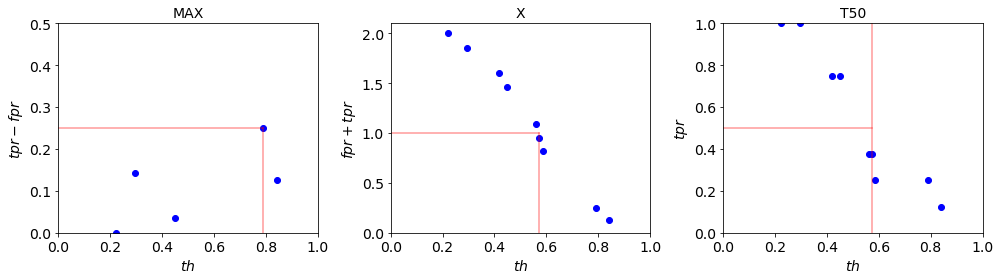
\includegraphics[width=\textwidth]{../plots_teoria/seleccion_umbrales_max_x_t50.png}
    \caption{}\label{fig:seleccion_umbrales_max_x_t50}
\end{figure}
Para el criterio MS, en cambio, por cada umbral que cambie \(fpr\) o \(tpr\) se
calcula una prevalencia (se descartan los casos indeterminados
por~\ref{ecuacion:acc_binaria}), y luego la mediana de todas ellas será la
predicción final del método.
\begin{figure}[H]
    \centerline{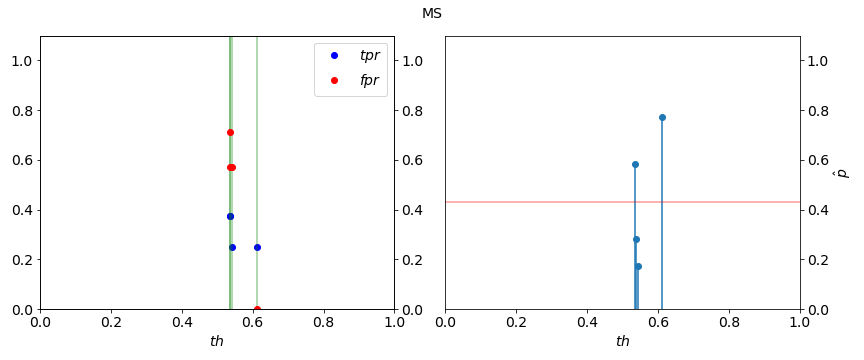
\includegraphics[width=0.75\textwidth]{../plots_teoria/seleccion_umbrales_ms.png}}
    \caption{}\label{fig:seleccion_umbrales_ms}
\end{figure}
Los resultados obtenidos fueron:
\begin{itemize}
    \item \(\hat p^{MAX}_{tst}(c=1) \approx  0.774\)
    \item \(\hat p^{X}_{tst}(c=1) \approx  0.282\)
    \item \(\hat p^{T50}_{tst}(c=1) \approx  0.282\)
    \item \(\hat p^{MS}_{tst}(c=1) \approx  0.433\)
\end{itemize}

\subsubsection{Esperanza-Maximización (EMQ)}\label{estimacion:emq}

Aunque este método se propuso originalmente para mejorar las probabilidades {\it
a posteriori\/} de modelos de clasificación bajo {\it dataset shift\/}
(ver~\ref{problema:cambios}), el mismo también sirve para mejorar la estimación
de prevalencias. También conocido como {\it SLD\/} por las iniciales de sus
autores, este método fue propuesto por~\citet{saerens2002adjusting} y aplica el
algoritmo de Esperanza-Maximización (EM)~\cite{dempster1977maximum}, un conocido
algoritmo iterativo para encontrar estimaciones de máxima verosimilitud de
parámetros (los valores de prevalencia de clase) para modelos que dependen de
variables no observadas (las etiquetas de clase). Esencialmente, {\it EMQ\/}
actualiza incrementalmente las probabilidades {\it a posteriori\/} utilizando
los valores de prevalencia de clases calculados en el último paso de la
iteración, y actualiza los valores de prevalencia de clases utilizando las
probabilidades {\it a posteriori\/} calculadas en el último paso de la
iteración, de forma mutuamente recursiva, y tomando como punto de partida un
valor determinado para la prevalencia de clases (generalmente el valor
correspondiente a la muestra de entrenamiento o una estimación {\it a priori\/}
dada por algún conocimiento de la muestra de prueba, aunque puede ser cualquier
otro valor), y repitiendo las iteraciones hasta alcanzar la convergencia.

\citet[Apéndice, p.23 a p.25]{saerens2002adjusting} demuestra, mediante el
Teorema de Bayes y el Teorema de probabilidad total, que el algoritmo de EM
aplicado a este problema resulta en los siguientes pasos (el paso 0 se aplica
una sola vez, luego se iteran el E y M):

\begin{enumerate}[leftmargin=*, labelindent=16pt]

    \item[\bf{0 -}] Inicialización de \(\hat p^{(0)}_{Y}(y=c_k)\), generalmente
    haciendo \(\hat p^{(0)}_{Y}(y=c_k) = \hat p_{tr}(c=c_k)\)

    \item[\bf{E -}] Esperanza: \hspace*{\fill}\makebox[4.5in][l]{\(\hat
    p^{(s)}_{Y|\boldsymbol{X}=\boldsymbol{x}_i}(y=c_k) = \dfrac{\dfrac{\hat
    p^{(s)}_{Y}(y=c_k)}{\hat p_{tr}(c=c_k)}s(\boldsymbol{x}_i, y=c_k)}{\sum
    \limits_{j=1}^{\#C} \dfrac{\hat p^{(s)}_{Y}(y=c_j)}{\hat
    p_{tr}(c=c_j)}s(\boldsymbol{x}_i, y=c_k)}\)}

    \item[\bf{M -}] Maximización: \hspace*{\fill}\makebox[4.5in][l]{\(\hat
    p^{(s+1)}_{Y}(y=c_k)=\dfrac{1}{m}\sum \limits_{i=1}^{m}\hat
    p^{(s)}_{Y|\boldsymbol{X}=\boldsymbol{x}_i}(y=c_k)\)}

\end{enumerate}

Finalmente, cuando se alcanza la convergencia, se obtiene: \(\hat p^{\it EMQ
\/}_{tst}(c=c_k) = \hat p_{Y}(y=c_k)\).

Aunque ya mencionamos que el modelo supone que las probabilidades {\it a
posteriori\/} de modelos de clasificación ya están calibradas, se ha estudiado
también que el método {\it EMQ\/} mejora las predicciones de cuantificación si
el clasificador utilizado está calibrado~\cite{esuli2020critical,
alexandari2020maximum}.

\paragraph{\it Ejemplo:\/} Comenzamos con la inicialización, dando en nuestro
caso como resultado \(\hat p^{(0)}_{Y}(y=1) = \hat p_{tr}(c=1) = 0.5\) y \(\hat
p^{(0)}_{Y}(y=0) = \hat p_{tr}(c=0) = 0.5\). En la primera iteración, para el
paso E queda \(\hat p^{(s=0)}_{Y|\boldsymbol{X}=\boldsymbol{x}_i}(y=c_k) =
s(\boldsymbol{x}_i, y=c_k)\) es decir, las mismas salidas del clasificador
calibrado. Luego, para el paso M, y al igual que en {\it PCC}, debemos promediar
cada salida individual del clasificador calibrado por cada una de las clases
existentes, quedando en nuestro caso \(\hat p^{(s=1)}_{Y}(y=1) = p^{\it
PCC\/}_{tst}(c=1) \approx 0.527\). Ahora, en el paso E de la segunda iteración,
se usará este último valor junto con los valores de prevalencia de la muestra de
entrenamiento para ajustar las salidas del clasificador calibrado. Por ejemplo,
para ajustar la salida del primer individuo correspondiente a la clase positiva,
sería: \(\hat p^{(s=1)}_{Y|\boldsymbol{X}=\boldsymbol{x}_i}(y=1) \approx
\dfrac{\dfrac{0.527}{0.5}0.539}{\dfrac{0.527}{0.5}0.539+\dfrac{0.473}{0.5}0.461}\).
Si continuamos repitiendo los pasos E y M de forma sucesiva, y definiendo un
criterio de corte para la convergencia (ya sea por máxima cantidad de
iteraciones o por un umbral de diferencia entre \(\hat p^{(s)}_{Y}(y=c_k)\) y
\(\hat p^{(s+1)}_{Y}(y=c_k)\)), se obtuvo \(p^{\it EMQ \/}_{tst}(c=1) \approx
0.164\).

\subsubsection{Usando la distancia de Hellinger en \(y\)
(HDy)}\label{estimacion:hdy}

\citet{gonzalez2013class} proponen dos métodos fundamentados en la comparación
de distribuciones. Aunque difieren en la manera de representar estas
distribuciones, ambos comparten un elemento esencial: emplean la distancia de
Hellinger como medida para cuantificar la disparidad entre ellas. El primer
método, conocido como {\it HDy}, es un método agregativo ya que emplea las
salidas del clasificador para describir las distribuciones tanto de la muestra
de entrenamiento como la de prueba. El método se basa en el cálculo de:
\begin{equation}\label{ecuacion:hdy}
    p^{\it HDy \/}_{tst}(c=1) = \argmin_{0 \leq \alpha \leq 1}{\text{HD}}(\alpha f_{tr}{(s(\boldsymbol{x},y=1|c=1))}+(1-\alpha) f_{tr}{(s(\boldsymbol{x},y=1|c=0))}, f_{tst}{(s(\boldsymbol{x},y=1))})
\end{equation}
donde:
\begin{equation}\label{ecuacion:hd}
    {\text{HD}}(P \parallel Q)= \frac{1}{\sqrt{2}}{\sqrt {\sum _{i=1}^{k}{({\sqrt {p_{i}}}-{\sqrt {q_{i}}})}^{2}}} \text{ con } P=(p_1,\dots,p_k), Q=(q_1,\dots,q_k)
\end{equation}
y \(f_{tr}(s)\) y \(f_{tst}(s)\) son las funciones de densidad de probabilidad
de las salidas del clasificador para la muestra de entrenamiento y de
evaluación, respectivamente. Estas densidades son aproximadas empíricamente
mediante histogramas, siendo \(k\) el número de {\it bins\/} utilizados. Dado
que el número de {\it bins\/} \(k\) podría tener un impacto significativo en la
estimación, normalmente se utiliza como estimador la mediana de la distribución
de los \(\alpha\) encontrados para un rango de \(k\).

El segundo método propuesto por~\citet{gonzalez2013class} pertenece a los
métodos no agregativos y será desarrollado en la correspondiente
sección~\ref{estimacion:no_agregativos}.

\paragraph{\it Ejemplo:\/} En las siguientes gráficas vemos cómo son las
estimaciones de tres distribuciones estimadas para el ejemplo, la gráfica de la
función de costo usada, y cómo el mínimo encontrado se usa para combinar las
distribuciones de entrenamiento y compararlas con la de prueba. En este caso, se
utilizó sólo \(k=200\).

\begin{figure}[h]
    \centering
    \begin{subfigure}[b]{\textwidth}
        \centering
        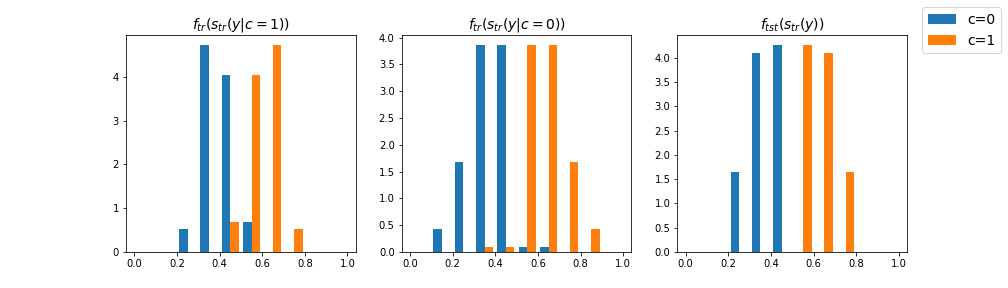
\includegraphics[width=\linewidth]{../plots_teoria/hdy_1.png}
    \end{subfigure}
    \begin{subfigure}[b]{0.4\textwidth}
        \centering
        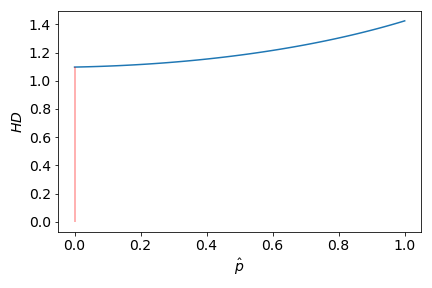
\includegraphics[width=\linewidth]{../plots_teoria/hdy_2.png}
    \end{subfigure}
    \begin{subfigure}[b]{\textwidth}
        \centering
        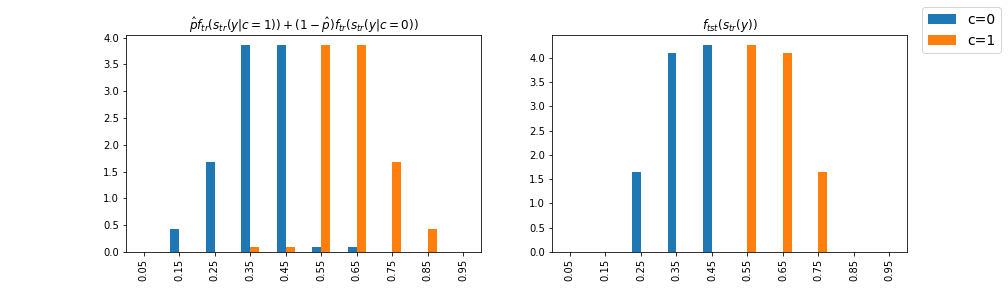
\includegraphics[width=\linewidth]{../plots_teoria/hdy_3.png}
    \end{subfigure}
    \hfill
\end{figure}

Se observa que el valor mínimo de HDy se da en \(p^{\it HDy \/}_{tst}(c=1) =
0.87\).

\subsection{Con clasificadores específicos}\label{estimacion:especificos}

Los métodos presentados anteriormente implican el uso de un clasificador, a
menudo seguido por una fase de ajuste para contrarrestar cualquier tendencia del
clasificador a subestimar o sobreestimar las proporciones de clases. Los
algoritmos discutidos en esta sección están específicamente diseñados con este
propósito en mente: durante el entrenamiento, tienen en cuenta que el modelo
será utilizado para cuantificar.

\subsubsection{Minimización de pérdida explícita (ELM)}\label{estimacion:elm}

Esta familia de métodos se aplican en principio a la cuantificación binaria,
pero son fácilmente extensibles a la cuantificación multiclase. La idea
propuesta por Esuli y Sebastiani~\cite{esuli2010sentiment} es seleccionar una
medida de rendimiento de cuantificación y entrenar un algoritmo de optimización
para construir el modelo óptimo según esa medida. Las diferencias entre ellos se
deben a la medida de rendimiento seleccionada y al algoritmo de optimización
utilizado.

Esuli y Sebastiani~\cite{esuli2010sentiment, esuli2014explicit,
esuli2015optimizing} proponen utilizar \({\it SVM
\/}_{perf}\)~\cite{joachims2005support} para optimizar la divergencia KL
-ver~\ref{evaluacion:dkl}-, mientras que~\citet{barranquero2015quantification}
también emplean \({\it SVM \/}_{perf}\) pero con una pérdida diferente,
argumentando que la cuantificación pura no considera la precisión del
clasificador subyacente (pudiendo generar un modelo que, aunque cuantifique
bien, clasifique mal). Para abordar esto, introducen la medida \(Q\), que
combina una evaluación de cuantificación con una evaluación de clasificación,
permitiendo un equilibrio entre ellas. Más recientemente Moreo y
Sebastiani~\cite{moreo2021re} reincorporaran la idea de utilizar \({\it SVM
\/}_{perf}\), pero sugieren usar las medidas de evaluación de error absoluto
(AE) y error absoluto negativo (RAE) -ver~\ref{evaluacion:ae}-.

Existen dos inconvenientes asociados con \({\it SVM \/}_{perf}\): podría
resultar en un modelo menos óptimo y no escala para grandes cantidades de datos
de entrenamiento. Para abordar estas limitaciones,~\citet{kar2016online}
proponen algoritmos de optimización estocástica. Además, plantean distintas
medidas multivariadas para evaluar el rendimiento de cuantificación. Siguiendo
esta línea,~\citet{sanyal2018optimizing} introducen una serie de algoritmos que
permiten el entrenamiento directo de redes neuronales profundas y la generación
de clasificadores no lineales. Estos métodos están diseñados para optimizar
funciones de pérdida de cuantificación como la divergencia KL.\@

\paragraph{\it Ejemplo:\/} A diferencia de los casos anteriores, aquí no usamos
el mismo clasificador con el que veníamos trabajando. En cambio, se ajusta un
nuevo clasificador pero con una función de pérdida más acorde al problema de
cuantificación. A modo de ejemplo, usaremos el método propuesto
por~\citet{esuli2010sentiment}, es decir, usando la divergencia KL como pérdida
y \({\it SVM \/}_{perf}\) como algoritmo de optimización. De esta forma,
obtuvimos un \(p^{{\it SVM \/}_{perf}, {\it KLD \/}}_{tst}(c=1) \approx 0.613\),
lo cual efectivamente implica una mejora del KLD con respecto a usar el
clasificador anterior con {\it CC}, ya que \({\it KLD \/}^{\it CC\/}_{tst}
\approx 0.887\) y \({\it KLD \/}^{{\it SVM \/}_{perf}, {\it KLD \/}}_{tst}
\approx 0.556\).

\section{Métodos No Agregativos}\label{estimacion:no_agregativos}

Hasta ahora, hemos utilizado métodos que agregan predicciones individuales de un
clasificador para poder cuantificar. Sin embargo, también es posible estimar
valores de prevalencia de clase sin generar decisiones binarias o probabilidades
{\it a posteriori\/} para cada ítem. Esta alternativa se fundamenta en el
principio de Vapnik, que sugiere resolver problemas directamente con la
información disponible en lugar de abordar un problema más general. En
cuantificación, esto significa que podemos estimar prevalencias de clase
directamente sin clasificar cada individuo.

\subsubsection{Usando la distancia de Hellinger en \(\boldsymbol{x}\)
(HDx)}\label{estimacion:hdx}

Este método está obviamente relacionado con {\it HDy\/} (\ref{estimacion:hdy}),
con la diferencia de considerar distribuciones de probabilidad
multidimensionales \(f(\boldsymbol{x})\) en lugar de distribuciones
unidimensionales \(f(s(\boldsymbol{x}))\). En vez de utilizar las salidas del
clasificador, se estiman, con los datos de entrenamiento, las funciones densidad
de las características de los individuos condicionadas a sus etiquetas.

Debido a la multidimensionalidad de \(\boldsymbol{x} \in
\mathbb{R}^d\),~\citet{gonzalez2013class} proponen minimizar el promedio de las
divergencias de Hellinger por cada \(\boldsymbol{x}^j\):

\begin{equation}\label{ecuacion:hdx}
    p^{\it HDx \/}_{tst}(c=1) = \argmin_{0 \leq \alpha \leq 1}{\frac{1}{d}\sum \limits_{j=1}^{d} \text{HD}}(\alpha f_{tr}({\boldsymbol{x^j}|c=1})+(1-\alpha) f_{tr}({\boldsymbol{x^j}|c=0}), f_{tst}({\boldsymbol{x^j}}))
\end{equation}

\paragraph{\it Ejemplo:\/} Repetimos el tipo de gráficos mostrados para  caso de
{\it HDy}, siendo en este caso \(k=10\).

\begin{figure}[h]
    \centering
    \begin{subfigure}[b]{\textwidth}
        \centering
        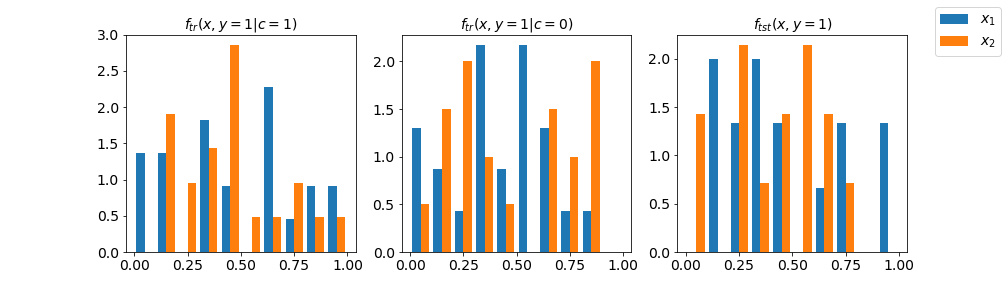
\includegraphics[width=\linewidth]{../plots_teoria/hdx_1.png}
    \end{subfigure}
    \begin{subfigure}[b]{0.4\textwidth}
        \centering
        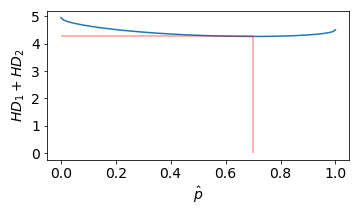
\includegraphics[width=\linewidth]{../plots_teoria/hdx_2.png}
    \end{subfigure}
    \begin{subfigure}[b]{\textwidth}
        \centering
        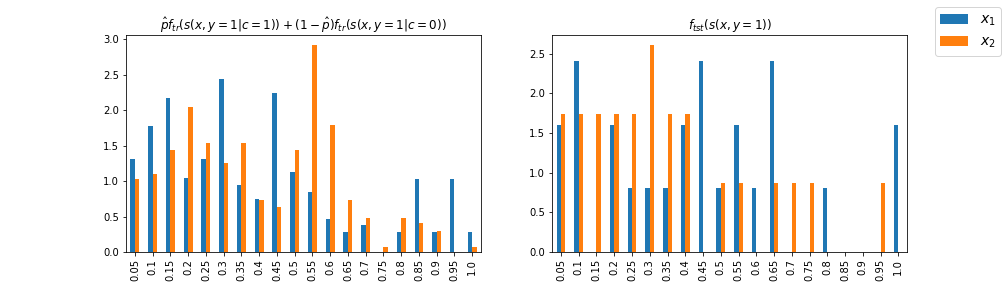
\includegraphics[width=\linewidth]{../plots_teoria/hdx_3.png}
    \end{subfigure}
    \hfill
\end{figure}

Se observa que el valor mínimo de HDx se da en \(p^{\it HDx \/}_{tst}(c=1) =
0.7\).

\subsubsection{Usando modelos generativos}\label{estimacion:generativos}

\citet{keith2018uncertainty} presentan un enfoque con modelos generativos para
estimar la prevalencia. Este método realiza una inferencia directa de la
prevalencia desconocida y aborda además el cálculo de intervalos de confianza
(IC)\footnote{Este enfoque es pionero en la cuantificación, ya que introduce un
modelo directo para el cálculo de los IC, los cuales eran estimados mediante
{\it bootstraping\/} en trabajos anteriores}.

Su propuesta, inspirada también en~\citet{saerens2002adjusting}, se basa en
modelar la distribución conjunta de las características de los individuos y sus
etiquetas, tanto en las datos de entrenamientos como en los de evaluación. En
base a esto se computa la verosimilitud marginal sobre \(\theta=p_{tst}\) para
obtener la distribución {\it a posteriori\/} de \(\theta\):

\begin{equation}\label{ecuacion:mll}
    {\it MLL\/}_{tst}(\theta) = \sum {\log \sum_{c \in C}{p_{tst}(\boldsymbol{x}_i, y_i=c | \theta)}}
\end{equation}

donde analizando para el caso binario, teniendo en cuenta que se asume
\(p_{tst}(\boldsymbol{x})=p_{tr}(\boldsymbol{x})\), y utilizando las funciones
de densidad de probabilidad de las características condicionadas a las etiquetas
estimadas con los datos de entrenamiento (\(p_{tr}(\boldsymbol{x}|y)\)), podemos
escribir:

\begin{equation}\label{ecuacion:mll_bin}
    {\it MLL\/}_{tst}(\theta) = \sum {\log \sum_{c \in C}{\theta p_{tr}(\boldsymbol{x}_i | y_i=1) + (1- \theta) p_{tr}(\boldsymbol{x}_i | y_i=0)}}
\end{equation}

Luego, para obtener la predicción se obtiene el máximo de la distribución. Es
decir, que al igual que el método {\it EMQ}, se busca maximizar la
verosimilitud, pero en este caso no necesariamente utilizando el algoritmo {\it
EM}. Esta función es unimodal en \(\theta \in [0,1]\). Como es cóncava y hay un
sólo parámetro, se pueden emplear muchas técnicas para encontrar la moda,
incluyendo {\it EM}, Newton-Rapshon o computacionalmente mediante una grilla de
valores.

\citet{keith2018uncertainty} proponen particularmente dos modelos generativos
enfocados en problemas de procesamiento de lenguaje ({\it MNB\/ y \it
Loglin\/}), al que llaman explícitos. Pero aún más interesante es el tercer
método que proponen, al que llaman {\it LR-Implicit}, el cual se basa en estimar
de forma implícita las \(p(\boldsymbol{x}|y)\) que obtendríamos con modelos
generativos mediante las \(p(y|\boldsymbol{x})\) que se obtienen con modelos
discriminativos, utilizando el Teorema de Bayes:

\begin{equation}\label{ecuacion:disc_gen}
    p_{disc}(y|\boldsymbol{x}) = \frac{p_{imp}(\boldsymbol{x}|y)p_{tr}(y)}{p(\boldsymbol{x})}
\end{equation}

Siendo \(p_{disc}(y|\boldsymbol{x})=h_{tr}(\boldsymbol{x})\), y sabiendo que al
querer maximizar~\ref{ecuacion:mll_bin} el valor de \(p(\boldsymbol{x})\) es
constante, entonces podemos utilizar en~\ref{ecuacion:mll_bin}:

\begin{equation}\label{ecuacion:disc_gen_2}
    p_{tr}(\boldsymbol{x}|y) \equiv h_{tr}(\boldsymbol{x}) / {\hat p_{tr}(y)}
\end{equation}

Un modelo generativo que utiliza un clasificador discriminativo como
intermediario para estimar \(p(\boldsymbol{x}|y)\) a partir de
\(p(y|\boldsymbol{x})\) (es decir, el método {\it LR-Implicit\/}) pertenece en
realidad a los métodos agregativos (mencionados en la
Sección~\ref{estimacion:agregativos}). No obstante, dado que el marco generativo
presentado por~\citet{keith2018uncertainty} solo requiere un modelo condicionado
por las etiquetas de clase, como ocurre con las versiones explícitas (usando los
modelos {\it MNB\/ y \it Loglin\/} como ejemplo), enmarcamos este método más
general dentro de los métodos no agregativos.

\paragraph{\it Ejemplo:\/} En este caso utilizaremos el método {\it LR-Implicit}
aplicado al clasificador con el que venimos trabajando. Utilizaremos el método
de grilla para buscar el máximo de la curva de \({\it MLL\/}_{tst}(\theta)\):
\begin{figure}[H]
    \centerline{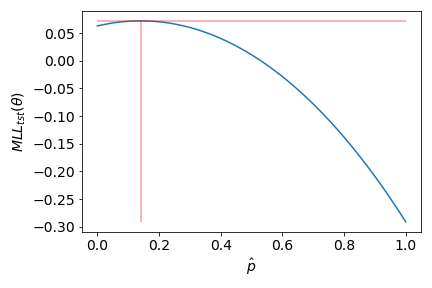
\includegraphics[width=0.5\textwidth]{../plots_teoria/lr_implicit.png}}
    \caption{}\label{fig:lr_implicit}
\end{figure}

Se observa que el valor mínimo de {\it LR-Implicit} se da en \(p^{\it
LR-Implicit \/}_{tst}(c=1) = 0.14\).

\chapter{Métodos de Evaluación}\label{evaluacion}

La evaluación de métodos de cuantificación es más compleja que en otros
problemas. En aprendizaje supervisado, típicamente se mide el rendimiento
estimando la probabilidad de predecir correctamente ejemplos individuales no
observados (sin condicionar -para la exactitud o {\it accuracy\/}- o
condicionando las probabilidades a las clases de pertenencia -para la
exhaustividad o {\it recall\/}- o predichas -para la precisión o {\it
precision\/}-). Sin embargo, en cuantificación, el rendimiento se evalúa para
conjuntos de datos. Esto implica que necesitamos una colección de muestras para
evaluar el rendimiento de un modelo. Dado un modelo $\overline{h}$, una función
de pérdida $L(\cdot, \cdot)$, y un conjunto de muestras de evaluación ${T_1,
\dots, T_s}$, el rendimiento de $\overline{h}$ es:

\begin{equation}
    Rendimiento(\overline{h}, L, {T_1, \dots , T_s}) = \frac{1}{s}
    \sum \limits_{j=1}^{s}L(\overline{h}, T_j)
    \label{ecuacion_rendimiento}
\end{equation}

Calcular la pérdida de un modelo sobre una muestra de prueba, $L(\overline{h},
T_j)$ no requiere de promediar sobre ejemplos individuales. Por ejemplo, en la
cuantificación binaria, sólo la prevalencia real $p$ y la prevalencia predicha
$\hat{p}$ se comparan por cada muestra.

En cuantificación, el problema de evaluación se relaciona con el cambio en la
distribución de datos entre la fase de entrenamiento y la de implementación del
modelo. Se requiere una colección de muestras de prueba variada y que represente
diversas distribuciones para evaluar correctamente el rendimiento del modelo y
evitar sesgos. Por esta razón, la mayoría de los experimentos reportados en la
literatura emplean conjuntos de datos tomados de otros problemas y se crean
conjuntos de prueba con cambios en las distribuciones creados artificialmente.
Este enfoque tiene la ventaja de que la cantidad del {\it dataset shift\/} se
puede controlar para estudiar el rendimiento de los modelos en diferentes
situaciones.

Las funciones de pérdida $L(\cdot, \cdot)$ serán elegidas de acuerdo al tipo de
problema y al objetivo particular de la aplicación. Como ya se mencionó, el
rendimiento de $\overline{h}$ será el promedio del resultado de la función de
pérdida por cada muestra de evaluación, de acuerdo a la
ecuación~\ref{ecuacion_rendimiento}. Se han propuesto en la literatura distintas
métricas de evaluación para problemas de {\it Single-Label Quantification
(SLQ)}. Estas también se pueden usar para {\it Binary Quantification (BQ)}, ya
que es un caso espacial del anterior, y para {\it Multi-Label Quantification},
ya que se pueden usar para cada $y \in C$. Esencialmente todas las medidas de
evaluación que se han propuesto son divergencias, es decir, medidas de cómo una
distribución difiere de otra. No se desarrollarán en esta tésis métricas para
{\it Ordinal Quantification\/} ni para {\it Regression Quantification }, ya que
no son útiles para nuestro objeto de estudio.

\section{Propiedades}\label{evaluacion:propiedades}

~\citet{sebastiani2020evaluation} define una serie de propiedades interesantes
para medidas de evaluación en {\it SLQ}. Un importante resultado de este
artículo es que ninguna medida de evaluación existente para {\it SLQ\/}
satisface todas las propiedades identificadas como deseables; aún así, se ha
demostrado que algunas medidas de evaluación son “menos inadecuadas” que otras.
Aquí mencionamos brevemente las cuatro propiedades principales que habría que
considerar en cada métrica $M$ a emplear (el resto son propiedas que suelen ser
satisfechas por todas las métricas).

\begin{itemize}
    \item {\bf Máximo (MAX)}: si $\exists \beta >0, \beta \in \mathbb{R}$ tal
    que por cada $c \in C$ y por cada $p$, (i) existe $\hat p$ tal que $M(p,
    \hat p) = \beta$, y (ii) para ninguna $\hat p$ se cumple que $M(p, \hat p) >
    \beta$. Si se cumple {\bf MAX}, la imagen de $M$ es independiente del
    problema, y esto permite juzgar si un valor dado significa un error de
    cuantificación alto o bajo. Si $M$ no cumple cumple {\bf MAX}, cada muestra
    de evaluación tendrá un peso distinto en el resultado final.
    \item {\bf Imparcial (IMP)}: si $M$ penaliza igualmente la subestimación de
    $p$ por una cantidad $a$ (es decir, con $\hat p = p - a$) o su
    sobreestimación por la misma cantidad $a$ (es decir, con $\hat p = p + a$).
    Si se cumple {\bf IMP}, la subestimación y la sobreestimación se consideran
    igualmente indeseables. Esto es generalmente lo deseable, a menos que exista
    una razón específica para no hacerlo.
    \item {\bf Relativo (REL)}: si $M$ penaliza más gravemente un error de
    magnitud absoluta $a$ (es decir, cuando $\hat p = p \pm a)$ si $p$ es menor.
    Por ejemplo, predecir $\hat p = 0.0101$ cuando $p = 0.0001$ es un error
    mucho más serio que predecir $\hat p = 0.1100$ cuando $p = 0.1000$.
    \item {\bf Absoluto (ABS)}: si $M$ penaliza un error de magnitud
    independientemente del valor de $p$. Mientras algunas aplicaciones requieren
    {\bf REL}, otras requieren {\bf ABS}. Si bien {\bf REL} y {\bf ABS} son
    mutuamente excluyentes, ninguna cubre el caso cuando $M$ considera un error
    de magnitud absoluta $a$ menos grave cuando $p$ es menor (como en el caso de
    la {\it distancia coseno\/}).
\end{itemize}

\section{Métricas}\label{evaluacion:metricas}

\subsection{Sesgo}

El sesgo o {\it bias\/} técnicamente no es una medida de evaluación para la
cuantificación, ya que no se aplica a toda una distribución $p$ sino solo a una
clase específica $c \in C$, y se define como:

\begin{equation}
    {\text{B}(c)} = \hat p(c) - p(c)
\end{equation}

Incluso usado en cuantificación binaria, se debe especificar a cuál de las
clases hacer referencia (en este caso, suele hacer referencia a la clase
positiva). Si se usa como un medida de evaluación para la cuantificación, un
problema con B es que promediar los puntajes de diferentes clases produce
resultados poco intuitivos, ya que el sesgo positivo de una clase y el sesgo
negativo de otra clase se anulan entre sí. El mismo problema ocurre cuando se
trata de la misma clase pero se promedia entre diferentes muestras. Como
resultado, esta medida se puede utilizar como mucho para determinar si un método
tiene una tendencia a subestimar o sobrestimar la prevalencia de una clase
específica (típicamente la clase minoritaria) en {\it BQ}, y no como una medida
de evaluación general para usar.

\subsection{Error Absoluto}

El error absoluto o {\it absolute error\/} es una de las medidas más empleadas
ya que, al ser simplemente la diferencia entre ambas magnitudes, es simple y
fácilmente interpretable.

\begin{equation}
    {\text{AE}(p, \hat p)} = \frac{1}{\#C}\sum \limits_{j=1}^{\#C}{|\hat p(c=c_j) - p(c=c_j)|}
\end{equation}

Como en este caso las diferencias positivas y negativas son igualmente
indeseables, promediar el AE entre varias clases, o varias muestras, no es
problemático. Como se muestra en~\cite{sebastiani2020evaluation}, AE cumple {\bf
IMP} y {\bf ABS} pero no cumple {\bf MAX} (ni tampoco {\bf REL}). Su rango va de
0 (mejor) a:
\begin{equation}
    z_{\text{AE}} = \frac{2(1-\displaystyle \min_{j\in\{1,\dots,\#C\}}p(c=c_j))}{\#C}
\end{equation}
(peor), por lo que su rango depende de la distribución de $p$ y de $\#C$.

\subsection{Error Absoluto Normalizado}

El error absoluto normalizado {\it normalised absolute error}, definido como:
\begin{equation}
    {\text{NAE}(p, \hat p)} = \frac{\text{AE}(p, \hat p)}{z_{\text{AE}}} = \frac{\sum \limits_{j=1}^{\#C}{|\hat p(c=c_j) - p(c=c_j)|}}{2(1-\displaystyle \min_{j\in\{1,\dots,\#C\}}p(c=c_j))}
\end{equation}
es una versión de AE que oscila entre 0 (mejor) y 1 (peor), por lo que cumple
{\bf MAX}. A pesar de su nombre, NAE no disfruta de {\bf ABS} (ni tampoco {\bf
REL}).

\subsection{Error Cuadrático}

El error cuadrático o {\it squared error}, definido como:
\begin{equation}
    {\text{SE}(p, \hat p)} = \frac{1}{\#C}\sum \limits_{j=1}^{\#C}{{(\hat p(c=c_j) - p(c=c_j))}^2}
\end{equation}
comparte los mismos pros y contras de AE, pero penalizando más cuanto mayor es
la diferencia entre el valor real y el predicho, por lo que se usa cuando se
quiere castigar los valores atípicos u {\it outliers}.

\subsection{Error Absoluto Relativo}

El error absoluto relativo o {\it relative absolute error\/} es una adaptación
del AE que impone {\bf REL} al hacer que AE sea relativo a $p$.

\begin{equation}
    {\text{RAE}(p, \hat p)} = \frac{1}{\#C}\sum \limits_{j=1}^{\#C}{\frac{|\hat p(c=c_j) - p(c=c_j)|}{p(c=c_j)}}
\end{equation}

RAE cumple {\bf IMP} y {\bf REL} pero no cumple {\bf MAX} (ni {\bf ABS}, a pesar
de su nombre). Su rango va de 0 (mejor) a:
\begin{equation}
    z_{\text{RAE}} = \frac{\#C - 1 + \frac {1 - \displaystyle \min_{j\in\{1,\dots,\#C\}}p(c=c_j)}{\displaystyle \min_{j\in\{1,\dots,\#C\}}p(c=c_j)}}{\#C}
\end{equation}
(peor), por lo que su rango depende de la distribución de $p$ y de $\#C$.

\subsection{Error Absoluto Relativo Normalizado}

El error absoluto relativo normalizado {\it normalised relative absolute error},
definido como:
\begin{equation}
    {\text{NRAE}(p, \hat p)} = \frac{\text{RAE}(p, \hat p)}{z_{\text{RAE}}} = \frac{\sum \limits_{j=1}^{\#C}{\frac{|\hat p(c=c_j) - p(c=c_j)|}{p(c=c_j)}}}{\#C - 1 + \frac {1 - \displaystyle \min_{j\in\{1,\dots,\#C\}}p(c=c_j)}{\displaystyle \min_{j\in\{1,\dots,\#C\}}p(c=c_j)}}
\end{equation}
es una versión de RAE que oscila entre 0 (mejor) y 1 (peor), por lo que cumple
{\bf MAX}. A pesar de su nombre, NRAE no disfruta de {\bf REL} (ni tampoco {\bf
ABS}).

Tanto RAE como NRAE no están definidas cuando sus denominadores sean nulos. Para
resolver este problema, se puede suavizar tanto $p(c=c_j)$ como $\hat p(c=c_j)$
mediante suavizado aditivo:
\begin{equation}
    \underline p(c=c_j) = \frac{\epsilon + p(c=c_j)}{\epsilon  \#C + \sum \limits_{j=1}^{\#C}{p(c=c_j)}}
\end{equation}
donde $\underline p(c=c_j)$ es la versión suavizada de $p(c=c_j)$ y el
denominador es solo un un factor de normalización (lo mismo para $\underline
{\hat p}(c=c_j)$).

\subsection{Divergencia de Kullback-Leibler}

Para distribuciones de probabilidad discretas $P$ y $Q$ definidas en el mismo
espacio muestral ${\mathcal {X}}$ su divergencia KL se define como:

\begin{equation}
    {\text{DKL}}(P\parallel Q)=\sum \limits_{x\in {X}}P(x)\log \left({\frac {P(x)}{Q(x)}}\right)
\end{equation}

En cuantificación, se quiere comparar la prevalencia real $p$ y la prevalencia
predicha $\hat{p}$, y el espacio muestral corresponde a las posibles clases, con
lo cuál será:
\begin{equation}
    {\text{DKL}}(p\parallel \hat{p}) = \sum \limits_{j=1}^{\#C}p(c=c_j)\log \left({\frac {p(c=c_j)}{\hat p(c=c_j)}}\right)
\end{equation}
que va de {0} (mejor) a {+$\infty$} (peor) -por lo tanto, no cumple con {\bf
MAX}-. Si bien esta medida es una distancia, no es una métrica verdadera, ya que
no obedece a la desigualdad del triángulo y no es simétrica. Además, es menos
interpretable que otras métricas de rendimiento y no está definido cuando
$\hat{p}$ es 0 o 1.

\subsection{Divergencia de Kullback-Leibler Normalizada}

Para suplir los problemas de DKL, se puede utilizar la función logística,
quedando:
\begin{equation}
    {\text{NDKL}}(p\parallel \hat{p}) = 2 \cdot \frac{e^{{\text{DKL}}(p\parallel \hat{p})}}{1+e^{{\text{DKL}}(p\parallel \hat{p})}}-1
\end{equation}
que también va de {0} (mejor) a {+$\infty$} (peor) -por lo tanto, si cumple con
{\bf MAX}-. Sin embargo, como se muestra en~\cite{sebastiani2020evaluation}, ni
DKL ni NDKL cumplen con {\bf IMP}, {\bf REL} y {\bf ABS}, lo que hace que su uso
como medidas de evaluación para cuantificación sea cuestionable, además de ser
dificiles de interpretar.

\section{Elección de la Métrica}\label{evaluacion:eleccion}

Es evidente que ninguna de las medidas propuestas hasta ahora es completamente
satisfactoria. DKL y NDKL son los menos satisfactorios y parecen fuera de
discusión. Respecto a los demás, el problema es que {\bf MAX} parece ser
incompatible con {\bf REL}/{\bf ABS}, y viceversa.

~\citet{sebastiani2020evaluation} sostiene que cumplir con {\bf REL} o {\bf ABS}
parece más importante que cumplir con {\bf MAX}, ya que reflejan las necesidades
de la aplicación; si no se satisfacen estas propiedades, se puede argumentar que
el error de cuantificación que se está midiendo está vagamente relacionado a lo
que el usuario realmente quiere. Si {\bf MAX} no está satisfecho, los resultados
obtenidos en muestras caracterizadas por diferentes distribuciones no serán
comparables. A pesar de esto, los resultados obtenidos por diferentes sistemas
en el mismo conjunto de muestras siguen siendo comparables.

Esto sugiere que AE, RAE y SE son las mejores medidas a elegir. Se debe preferir
AE cuando un error de estimación de una magnitud absoluta dada debe considerarse
más grave cuando la verdadera prevalencia de la clase afectada es menor. RAE
debe ser elegido cuando un error de estimación de una magnitud absoluta dada
tiene el mismo impacto independientemente de la verdadera prevalencia de la
clase afectada. Si se quiere penalizar mayormente errores atípicos, considerando
mucho más graves a los errores cuanto mayor es la diferencia entre el valor real
y el predicho, entonces SE es la métrica más conveniente.

\section{Protocolos}\label{evaluacion:protocolos}

Mientras que en la clasificación, un conjunto de datos de tamaño $k$ proporciona
$k$ puntos de evaluación, para la cuantificación, el mismo conjunto solo
proporciona $1$ punto. Evaluar algoritmos de cuantificación es por lo tanto un
reto, debido a que la disponibilidad de datos etiquetados con fines de prueba es
más restringido. Hay principalmente dos protocolos experimentales que se han
tomado para tratar con este problema: el Protocolo de Prevalencia Natural ({\it
NPP\/}) y el Protocolo de Prevalencia Artificial ({\it APP\/}).

\begin{itemize}
    \item {\it NPP\/}: Consiste en, una vez entrenado un cuantificador, tomar un
    conjunto de prueba (no observado en el entrenamiento) lo suficientemente
    grande, dividirlo en un número de muestras de manera uniformemente
    aleatoria, y llevar a cabo la evaluación individualmente en cada muestra.
    \item {\it APP\/}: Consiste en, previo al entrenamiento, tomar un conjunto
    de datos, dividirlo en un conjunto de entrenamiento y en un conjunto de
    evaluación de manera aleatoria, y realizar experimentos repetidos en los que
    la prevalencia del conjunto de entrenamiento o la prevalencia del conjunto
    de prueba de una clase se varía artificialmente a través del submuestreo.
\end{itemize}

Ambos protocolos tienen diferentes pros y contras. Una ventaja de {\it APP\/} es
que permite crear muchas puntos de prueba de la misma muestra. Además, {\it
APP\/} permite simluar distintos {\it Prior probability shift}, mientras que con
{\it NPP\/} se estaría evaluando sólo con las distribuciones originales de los
datos de entrenamiento y prueba. Sin embargo, una desventaja de {\it APP\/} es
que puede no saberse cuán realistas son estas diferentes situaciones en la
aplicación real, por lo que se podría estar destinando recursos a una evaluación
errónea o pobre. Una solución intermedia podría ser utilizar un protocolo que
utilice conocimientos previos sobre la distribución de prevalencias “probables”
que se podría esperar encontrar en el dominio específico en cuestión.

\chapter{Experimentos}\label{experimentos}

En esta sección se evaluarán todos los métodos mencionados en el
Capítulo~\ref{estimacion} mediante nuevos casos de ejemplo simulados. Dicha
evaluación se basará en las medidas de evaluación elegidas
en~\ref{evaluacion:eleccion} (RAE, AE y SE) además del error. Además, la
simulación se basará en el protocolo {\it APP\/} definido
en~\ref{evaluacion:protocolos}. No se realizará el proceso de selección de
modelos mencionado en~\ref{evaluacion:seleccion} ya que el objetivo de estos
experimentos no es el de buscar los mejores cuantificadores para los casos de
ejemplo, sino hacer una comparación de los mismos frente a iguales condiciones
(hiperparámetros por defecto, mismo clasificador, etc.). Finalmente, se elaboran
conclusiones en base a los resultados y se comparan con los resultados de otros
trabajos~\cite{moreo2021re, moreo2022tweet, moreo2021quapy, tasche2016does,
schumacher2021comparative}.

\section{Simulación}\label{experimentos:simulacion}

\subsection{Poblaciones}\label{experimentos:poblaciones}

La simulación consiste, en primer lugar, en generar dos poblaciones sintéticas
de datos. Al igual que en~\ref{estimacion:ejemplo}, para sintetizar los datos se
utilizó el algoritmo propuesto por~\citet{Guyon2003DesignOE} mediante la
función~\href{https://scikit-learn.org/stable/modules/generated/sklearn.datasets.make_classification.html}{{\it
make\_classification}} de {\it scikit-learn}. En este caso, se crearon dos
poblaciones, {\it F\/} (fácil) y {\it D\/} (difícil), cuyos argumentos de
creación son (los parámetros no mencionados usan sus valores por defecto):
\begin{center}
    \begin{tabular}{l|ll|ll}
        \cline{2-3}
        & \multicolumn{2}{l|}{Población} & & \\ \cline{2-3} &
        \multicolumn{1}{l|}{F}     & D     & &  \\ \cline{1-3}
        \multicolumn{1}{|l|}{n\_samples}
        & \multicolumn{1}{l|}{51000} & 51000 &  &  \\
        \multicolumn{1}{|l|}{n\_features}    & \multicolumn{1}{l|}{2}     & 100
        & &  \\
        \multicolumn{1}{|l|}{n\_informative} & \multicolumn{1}{l|}{2}     & 5 &
        &  \\
        \multicolumn{1}{|l|}{n\_redundant}   & \multicolumn{1}{l|}{0}     & 15 &
        &  \\
        \multicolumn{1}{|l|}{n\_repeated}    & \multicolumn{1}{l|}{0}     & 15 &
        &  \\
        \multicolumn{1}{|l|}{flip\_y}        & \multicolumn{1}{l|}{0}     & 0 &
        &  \\
        \multicolumn{1}{|l|}{class\_sep}     & \multicolumn{1}{l|}{0.6}   & 0.2
        &  &  \\ \cline{1-3}
    \end{tabular}
    \captionof{table}{Poblaciones}\label{experimentos:tabla_poblaciones}
\end{center}

La elección de estos valores tiene como objetivo generar una población fácil de
clasificar y con características de baja dimensionalidad, y otra más difícil y
con alta dimensionalidad, para probar bajo estas dos condiciones cada método.
Además, al usar los parámetros {\it n\_classes\/} y {\it weights\/} por defecto,
estaremos generando datasets binarios y perfectamente balanceados.

\subsection{Datasets}\label{experimentos:datasets}

Tenemos entonces dos poblaciones sintéticas, cada una de 51000 individuos.
Luego, procedemos a sub-dividir ambas poblaciones de forma estratificada (es
decir, manteniendo la proporción de clases balanceadas) para crear los datasets
de entrenamiento y de prueba en cada población. Dichos datasets son de 50000 y
1000 individuos respectivamente.

Siguiendo el protocolo {\it APP\/} ya mencionado, la simulación consistió en
muestrear de forma iterativa el dataset de entrenamiento de cada población con
distintos tamaños de muestra (500 y 5000), distintas prevalencias\footnote{Para
evitar repeticiones, cuando mencionemos prevalencia en estos casos se hará
referencia siempre a la clase positiva.} (0.01, 0.25, 0.5, 0.75 y 0.99) y de
forma repetida (5 veces) -es decir, un total de 50 muestras distintas-. Luego,
por cada muestra de entrenamiento, a su vez, se muestreo de forma iterativa el
dataset de evaluación. En este caso también se tomaron distintos tamaños de
muestra (10 y 100), distintas prevalencias (0, 0.2, 0.5, 0.8 y 1.0 para las
muestras de tamaño n=10, y 0.01, 0.25, 0.5, 0.75 y 0.99 para las muestras de
tamaño n=100) y de forma repetida (5 veces) -50 muestras de prueba por cada
muestra de entrenamiento-.
\begin{center}
    \begin{tabular}{l|cccc|}
        \cline{2-5}
        & \multicolumn{4}{c|}{Dataset} \\
        \cline{2-5} &
        \multicolumn{2}{c|}{Train}
        & \multicolumn{2}{c|}{Test} \\
        \hline
        \multicolumn{1}{|l|}{n\_samples}  & \multicolumn{1}{c|}{500} &
        \multicolumn{1}{c|}{5000}                    &
        \multicolumn{1}{c|}{10}
        & 100 \\ \hline
        \multicolumn{1}{|l|}{prev}        &
        \multicolumn{2}{c|}{\begin{tabular}[c]{@{}c@{}}0.01\\ 0.25\\ 0.5\\
        0.75\\ 0.99\end{tabular}} &
        \multicolumn{1}{c|}{\begin{tabular}[c]{@{}c@{}}0\\ 0.2\\ 0.5\\ 0.8\\
        1.0\end{tabular}} & \begin{tabular}[c]{@{}c@{}}0.01\\ 0.25\\ 0.5\\
        0.75\\ 0.99\end{tabular} \\ \hline
        \multicolumn{1}{|l|}{n\_repetitions} & \multicolumn{2}{c|}{5} &
        \multicolumn{2}{c|}{5} \\ \hline
    \end{tabular}
    \captionof{table}{Datasets}\label{experimentos:tabla_datasets}
\end{center}

\subsection{Cuantificación}\label{experimentos:cuantificacion}

Por cada muestra de entrenamiento, se procede a ajustar cada uno de los métodos
a evaluar. Empezando por los métodos agregativos que utilizan clasificadores
generales (\ref{estimacion:generales}), tenemos los que requieren como entrada
las etiquetas de las clases predichas (es decir, que usan clasificadores duros).
En nuestro caso, estos métodos son el {\it CC\/} y el {\it ACC}. Es decir, que
primero debemos ajustar un modelo de clasificación. En esta simulación hemos
utilizado dos modelos distintos, un modelo de regresión logística y el
clasificador de XGBoost, con la idea de probar un modelo simple y uno complejo,
con el objetivo de determinar si la complejidad del modelo mejora o no la
cuantificación. En este caso no es necesario calibrarlos ya que usaremos
solamente las etiquetas predichas. Para sus hiperparámetros usaremos los valores
por defecto de las librerías {\it scikit-learn\/} y {\it xgboost\/}
respectivamente.
\begin{center}
    \begin{tabular}{|lc|}
        \hline
        \multicolumn{2}{|c|}{Clasificación}                     \\ \hline
        \multicolumn{1}{|c|}{Modelo}             & Complejidad  \\ \hline
        \multicolumn{1}{|l|}{LogisticRegression} & Baja         \\
        \multicolumn{1}{|l|}{XGBoost}            & Alta         \\ \hline
    \end{tabular}
\captionof{table}{Modelos de
clasificación}\label{experimentos:tabla_clasificacion}
\end{center}

En cambio, para los métodos agregativos que utilizan clasificadores generales
pero que requieren como entrada las probabilidades {\it a posteriori\/} de
pertenencia a cada clase (es decir, clasificadores blandos), debemos no solo
ajustar los modelos de clasificación, sino que también conviene calibrarlos (ya
que es un supuesto de estos métodos). En nuestro caso, estos métodos son el {\it
PCC}, {\it PACC}, {\it EMQ\/} y {\it HDy}. Con respecto a los algoritmos de
calibración, utilizaremos los cuatro métodos para modelos binarios propuestos
por~\citet{guo2017calibration} y mencionados en el
Apéndice~\ref{appendix:calibracion}, además de probar también los clasificadores
sin calibrar. Como los métodos de calibración requieren utilizar validación
cruzada para ajustar sus parámetros, utilizaremos el método de {\it held-out},
es decir que destinaremos una porción (20\%) del dataset de entrenamiento para
ello.
\begin{center}
    \begin{tabular}{|lc|}
        \hline
        \multicolumn{2}{|c|}{Calibración}                    \\ \hline
        \multicolumn{1}{|c|}{Método}              & Held-out \\ \hline
        \multicolumn{1}{|l|}{No Calibration}      & 0\%      \\
        \multicolumn{1}{|l|}{Histogram Binning}   & 20\%     \\
        \multicolumn{1}{|l|}{Isotonic Regression} & 20\%     \\
        \multicolumn{1}{|l|}{BBQ}                 & 20\%     \\
        \multicolumn{1}{|l|}{Platt Scaling}       & 20\%     \\ \hline
    \end{tabular}
    \captionof{table}{Modelos de
    calibración}\label{experimentos:tabla_calibracion}
\end{center}

Para los métodos agregativos que utilizan clasificadores específicos
(\ref{estimacion:especificos}) -en nuestro caso, únicamente el método {\it
ELM\/}-, debemos también ajustar un modelo de clasificación previo a la
cuantificación, pero en este caso no utilizaremos los nombrados
en~\ref{experimentos:tabla_clasificacion}, sino uno optimizado para ser
utilizado en cuantificación. En este caso usaremos, al igual que en el
Capítulo~\ref{evaluacion}, el clasificador \({\it SVM \/}_{perf}\), pero esta
vez optimizado no solo para KLD, sino también AE y RAE.

Para los modelos no agregativos (\ref{estimacion:no_agregativos}), no se usan
modelos de clasificación, y por lo tanto tampoco se calibran; simplemente se
aplica directamente el método de cuantificación. En nuestro caso, para este
grupo usaremos solo el método {\it HDx}, ya que no usaremos modelos de
clasificación generativos explícitos. Sin embargo, sí usaremos el método {\it
LR-Implicit}, el cual, como bien dijimos, se debe considerar en realidad un
método agregativo, y así lo haremos en las simulaciones.

Cabe mencionar que para los métodos de cuantificación que requieren de
validación cruzada para estimar sus parámetros internos también utilizaremos el
método de {\it held-out}, destinando otra porción (20\%) del dataset de
entrenamiento para ello.
\begin{center}
    \begin{tabular}{|lc|}
        \hline
        \multicolumn{2}{|c|}{Cuantificación}                              \\
        \hline
        \multicolumn{1}{|c|}{Método}      & \multicolumn{1}{c|}{Held-out} \\
        \hline
        \multicolumn{1}{|l|}{CC}          & \multicolumn{1}{c|}{0\%}      \\
        \multicolumn{1}{|l|}{ACC}         & \multicolumn{1}{c|}{20\%}     \\
        \multicolumn{1}{|l|}{PCC}         & \multicolumn{1}{c|}{0\%}      \\
        \multicolumn{1}{|l|}{PACC}        & \multicolumn{1}{c|}{20\%}     \\
        \multicolumn{1}{|l|}{TH\_MAX}     & \multicolumn{1}{c|}{20\%}     \\
        \multicolumn{1}{|l|}{TH\_X}       & \multicolumn{1}{c|}{20\%}     \\
        \multicolumn{1}{|l|}{TH\_T50}     & \multicolumn{1}{c|}{20\%}     \\
        \multicolumn{1}{|l|}{TH\_MS}      & \multicolumn{1}{c|}{20\%}     \\
        \multicolumn{1}{|l|}{EMQ}         & \multicolumn{1}{c|}{0\%}      \\
        \multicolumn{1}{|l|}{HDy}         & \multicolumn{1}{c|}{20\%}     \\
        \multicolumn{1}{|l|}{HDx}         & \multicolumn{1}{c|}{0\%}      \\
        \multicolumn{1}{|l|}{ELM-SVMperfKLD}  & \multicolumn{1}{c|}{0\%} \\
        \multicolumn{1}{|l|}{ELM-SVMperfAE}   & \multicolumn{1}{c|}{0\%} \\
        \multicolumn{1}{|l|}{ELM-SVMperfRAE}  & \multicolumn{1}{c|}{0\%} \\
        \multicolumn{1}{|l|}{LR-Implicit} & \multicolumn{1}{c|}{0\%}      \\
        \hline
    \end{tabular}
    \captionof{table}{Modelos de
    cuantificación}\label{experimentos:tabla_cuantificacion}
\end{center}

Finalmente, una vez ajustado el método de cuantificación para una muestra de
entrenamiento, se procede a tomar una muestra de prueba (recordando que
probaremos con distintos tamaños de muestra, prevalencia y repitiendo el
muestreo) y estimar su prevalencia.

Para la implementación de los métodos de cuantificación en la simulación se
utilizó la librería \href{https://github.com/HLT-ISTI/QuaPy}{{\it
Quapy}}~\cite{moreo2021quapy} (\url{https://github.com/HLT-ISTI/QuaPy}), excepto
para el método \href{https://github.com/slanglab/freq-e}{{\it
LR-Implicit}}~\cite{keith2018uncertainty}, para el cual se empleó el código
provisto por los autores (\url{https://github.com/slanglab/freq-e}). Para la
implementación de los modelos de calibración utilizamos la
librería~\href{https://github.com/EFS-OpenSource/calibration-framework}{{\it
net:cal}}~\cite{kuppers2020multivariate}
(\url{https://github.com/EFS-OpenSource/calibration-framework}).

\subsection{Evaluación}\label{experimentos:evaluación}

Como ya se mencionó, se realizó la evaluación en base a las medidas elegidas
en~\ref{evaluacion:eleccion}, es decir, se utilizaron RAE, AE y SE. La
evaluación se hizo según distintos criterios, agrupando los resultados en base a
estos criterios y calculando su intervalo de confianza del 95\%. Además, en los
casos que corresponda, usaremos también la medida de clasificación F1 y la
medida de calibración ECE para elaborar conclusiones.

\section{Conclusiones}\label{experimentos:conclusiones}

Empezamos por analizar el rendimiento de los cuantificadores en general. En la
tabla~\ref{experimentos:by_quantifier} se muestran los resultados de las
estimaciones de las medidas RAE, AE y SE para cada cuantificador usado en la
simulación. Los métodos basados en selección de umbrales ({\it TH\/}), {\it
PACC\/}, {\it LR-Implicit\/} y {\it EMQ\/} son los que en general mejor
desempeño tienen, mientras que los basados en minimización de pérdida explícita
({\it ELM\/}) son los peores. Estos resultados son congruentes con los
de~\citet{schumacher2021comparative} (en donde {\it TH\_MS\/} es el método con
mejor AE), los de~\citet{moreo2021re} (que afirma que {\it PACC\/} es el mejor
método dentro de las variantes de {\it CC\/}), los de~\citet{moreo2021quapy}
(donde {\it EMQ\/} resultó el método con mejor AE), los
de~\citet{moreo2022tweet} (donde también {\it EMQ\/} y {\it PACC\/} resultaron
los mejores métodos evaluados con AE) y los de~\citet{tasche2016does} (que
concluye que los métodos {\it CC\/} y {\it PCC\/} son limitados frente a {\it
ACC\/} y {\it PAC\/}).

Si queremos ver si los métodos sobre o sub estiman las prevalencias, debemos
entonces analizar los errores (y principalmente, el sesgo o {\it bias\/}).
Podemos observar en la figura~\ref{fig:global_bias_by_quantifier} que {\it
HDy\/} está levemente sesgado a subestimar, mientras que el resto de los métodos
no presentan, en general, un sesgo marcado. Sin embargo, si analizamos el sesgo
en función de la verdadera prevalencia en la muestra de prueba
(figura~\ref{fig:diagonal_by_cuantificator}), todos los métodos si tienen un
sesgo en favor de la clase minoritaria (excepto justamente para algunos valores
de {\it HDy\/}).

\begin{figure}[!tph]
    \centering
    \centerline{\includegraphics[width=0.9\textwidth]{../experiments/plots/global_bias_by_quantifier.png}}
    \caption{Error por método de
    cuantificación}\label{fig:global_bias_by_quantifier}
\end{figure}
\begin{figure}[!tph]
    \centering
    \centerline{\includegraphics[width=0.6\textwidth]{../experiments/plots/diagonal_by_cuantificator.png}}
    \caption{Prevalencia estimada por método de cuantificación según prevalencia
    de prueba}\label{fig:diagonal_by_cuantificator}
\end{figure}

Por otro lado, también verificamos algunas de los resultados que eran de
esperarse:
\begin{itemize}[noitemsep]
    \item Para los métodos de cuantificación agregativos con clasificadores
    generales (\ref{estimacion:generales}), a mejor desempeño en la
    clasificación (evaluado con la medida F1), mejor desempeño en la
    cuantificación (tabla~\ref{experimentos:by_classifier}).
    \item A menor cantidad de características y mayor separación entre clases en
    las poblaciones, mejor rendimiento de cuantificación
    (tabla~\ref{experimentos:by_population}).
    \item A mayor tamaño en muestra de entrenamiento, mejor rendimiento de
    cuantificación (tabla~\ref{experimentos:by_train_sample_size}) (coincide con
    los resultados de~\citet{schumacher2021comparative}).
\end{itemize}

Si analizamos según el tamaño de la muestra de evaluación
(tabla~\ref{experimentos:by_test_sample_size}), teniendo que para cada tamaño
utilizamos distintas posibles prevalencias como definimos en la
tabla~\ref{experimentos:tabla_datasets}, y recordando que los valores de las
medidas de evaluación dependen de los mínimos valores posibles de las
prevalencias de prueba (ecuaciones~\ref{evaluacion:eq_zae}
y~\ref{evaluacion:eq_zrae}), entendemos entonces la diferencia de resultados en
las medidas entre los distintos tamaños de muestra.

Vemos también que cuanto más balanceada sea la muestra de entrenamiento, mejores
resultados de cuantificación se obtienen (tabla~\ref{experimentos:by_train_prev}
y figuras~\ref{fig:global_bias_by_train_prev}
y~\ref{fig:diagonal_by_train_prev}). Este es un dato bastante interesante, ya
que implicaría que podríamos aplicar en cuantificación las mismas técnicas de
balance de clases que se usan en problemas de clasificación para tratar de
conseguir mejores resultados que si usáramos datos desbalanceados. También vemos
como la prevalencia de la muestra de entrenamiento influye en el sesgo del
cuantificador, tendiendo en general a sobrestimar la clase mayoritaria. En la
figura~\ref{fig:diagonal_by_quantifier_by_train_prev} podemos ver estos
resultados desagregados por método de cuantificación.

\begin{figure}[!tph]
    \centering
    \centerline{\includegraphics[width=0.6\textwidth]{../experiments/plots/global_bias_by_train_prev.png}}
    \caption{Error por prevalencia de
    entrenamiento}\label{fig:global_bias_by_train_prev}
\end{figure}
\begin{figure}[!tph]
    \centering
    \centerline{\includegraphics[width=0.5\textwidth]{../experiments/plots/diagonal_by_train_prev.png}}
    \caption{Prevalencia estimada por prevalencia de entrenamiento según
    prevalencia de prueba}\label{fig:diagonal_by_train_prev}
\end{figure}

\begin{figure}[H]
    \centering
    \begin{subfigure}[b]{.475\textwidth}
        \centering
        \includegraphics[width=\linewidth]{../experiments/plots/diagonal_by_cuantificator_0.01.png}\quad
    \end{subfigure}
    \begin{subfigure}[b]{.475\textwidth}
        \centering
        \includegraphics[width=\linewidth]{../experiments/plots/diagonal_by_cuantificator_0.25.png}\quad
    \end{subfigure}
    \medskip
    \begin{subfigure}[b]{.475\textwidth}
        \centering
        \includegraphics[width=\linewidth]{../experiments/plots/diagonal_by_cuantificator_0.50.png}
    \end{subfigure}
    \begin{subfigure}[b]{.475\textwidth}
        \centering
        \includegraphics[width=\linewidth]{../experiments/plots/diagonal_by_cuantificator_0.75.png}\quad
    \end{subfigure}
    \begin{subfigure}[b]{.65\textwidth}
        \centering
        \includegraphics[width=\linewidth]{../experiments/plots/diagonal_by_cuantificator_0.99.png}
    \end{subfigure}
    \medskip
    \hfill
    \caption{Prevalencia estimada por método de cuantificación según prevalencia
    de prueba, para distintas prevalencias de
    entrenamiento}\label{fig:diagonal_by_quantifier_by_train_prev}
\end{figure}

Con respecto al balance en la muestra de prueba
(tabla~\ref{experimentos:by_test_prev}), debemos volver a mencionar el
comentario en referencia a los distintos valores de prevalencia para los
distintos posibles tamaños de muestra. De todas formas, llama la atención que
las medidas de evaluación son mejores cuando el desbalance de clases lleva a la
clase positiva a ser la minoritaria. Esto se debe a que los métodos de
cuantificación binaria basados en la estimación del {\it fpr\/} y {\it tpr\/}
({\it ACC}, {\it PACC}, y {\it TH\/}) no son simétricos en cuanto a las clases
positivas y negativas, sino que son sensibles a si la clase mayoritaria es una u
otra.

Si tenemos en cuenta la diferencia absoluta entre las prevalencias de la muestra
de entrenamiento y la de prueba (tabla~\ref{experimentos:by_abs_dataset_shift}),
vemos que también en general (y como quizás era esperable de forma intuitiva), a
menor diferencia, mejor rendimiento. Sin embargo, llama la atención cuan
dinámico es este comportamiento según el método de cuantificación
(tabla~\ref{experimentos:by_abs_dataset_shift_and_quantificator}). En general,
los métodos que mejor funcionan cuando el {\it dataset shift\/} es bajo son los
que peor funcionan cuando es alto. A pesar de que en~\citet{moreo2022tweet}
y~\citet{moreo2021quapy} el método {\it EMQ\/} es el de mejor rendimiento para
los casos de mayor {\it dataset shift}, en nuestras simulaciones fue {\it
TH\_T50\/} el método con mejor evaluación ante estos casos.

\begin{figure}[!tph]
    \centering
    \centerline{\includegraphics[width=0.9\textwidth]{../experiments/plots/global_bias_by_calibration.png}}
    \caption{Error por método de
    calibración}\label{fig:global_bias_by_calibration}
\end{figure}
\begin{figure}[!tph]
    \centering
    \centerline{\includegraphics[width=0.7\textwidth]{../experiments/plots/diagonal_by_calibration.png}}
    \caption{Prevalencia estimada por método de calibración según prevalencia en
    muestra de prueba}\label{fig:diagonal_by_calibration}
\end{figure}

Analizando ahora la influencia de la calibración en la cuantificación, la
calibración por regresión isotónica lleva una leve ventaja en el rendimiento de
la cuantificación en general (considerando solo métodos de cuantificación
agregativos con clasificadores generales y blandos)
(tabla~\ref{experimentos:by_calibration} y
figuras~\ref{fig:global_bias_by_calibration} y
~\ref{fig:diagonal_by_calibration}), aunque llamativamente no presenta ventajas
en cuánto a la medidas de clasificación (F1) ni de calibración (ECE).

Si tenemos en cuenta tanto el método de cuantificación como el de calibración
(en los casos que aplique)
(tabla~\ref{experimentos:by_quantifier_and_calibration} y
figura~\ref{fig:global_bias_by_quantifier_and_calibration}), se observa que {\it
LR-Implicit}, {\it EMQ} y {\it PACC} en los casos de calibración isotónica y de
no calibración se vuelven más competitivos frente a los métodos {\it TH}.

\begin{figure}[!tph]
    \centering
    \centerline{\includegraphics[width=\textwidth]{../experiments/plots/global_bias_by_quantifier_and_calibration.png}}
    \caption{Error por método de calibración y
    cuantificación}\label{fig:global_bias_by_quantifier_and_calibration}
\end{figure}

Sin embargo, también notamos que esta mejora en la cuantificación mediante la
calibración surge cuanto más desbalanceados estén los datos de entrenamiento, no
habiendo mejoras significativas cuando están balanceados
(tabla~\ref{experimentos:by_train_prev_and_calibration}).



\appendix

\chapter{Calibración}\label{appendix:calibracion} 

En problemas de clasificación, el subproblema de la predicción de estimaciones
de probabilidad representativas de las probabilidades verdaderas es conocido
como calibración. En los sistemas del mundo real, los clasificadores no sólo
deben ser precisos, sino que también deben indicar cuando es probable que sean
incorrectos. Es decir, deben estimar su nivel de incertidumbre o confiabilidad.
En otras palabras, las probabilidades asociadas con la etiquetas de clase
predichas deben reflejar su verosimilitud real.

Uno de los casos en donde se debe contemplar este problema es en la toma de
decisiones (es decir, en casi toda aplicación real). Por ejemplo, en sistemas
utilizados para la salud, un diagóstico con un bajo nivel de confianza puede
significar realizar otro tipo de chequeo. A su vez, las estimaciones de
probabilidad, pueden ser utilizadas para ser incorporadas en otro modelo
probabilístico. Por ejemplo, se podrían combinar distintas salidas de distintos
modelos de forma ponderada para obtener una predicción más robusta frente los
casos en donde cada modelo individual falla.

La mayoría de los métodos de aprendizaje supervisado producen clasificadores que
generan puntuaciones \(s(x)\) que se pueden utilizar para ranquear los ejemplos
en el conjunto de pruebas de la etiqueta más probable a la menos probable de una
clase \(c\). Es decir, para dos ejemplos \( \mathbf{x}_1\) y \( \mathbf{x}_2\),
si \(s( \mathbf{x}_1) < s( \mathbf{x}_2)\) entonces \(\mathbb{P}(c|x) <
\mathbb{P}(c|y)\). Sin embargo, la clasificación según el rango de la
probabilidad de pertenencia a una clase no es suficiente. Lo que se necesita es
una estimación precisa de la probabilidad de que cada ejemplo de prueba sea un
miembro de la clase de interés.

El modelo de regresión logística es un caso especial ya que está bien calibrado
por diseño dado que su función objetivo minimiza la función de pérdida
logarítmica o {\it log-loss\/}~\cite{morrison2013tutorial}. Sin  embargo, si no
se cuenta con un conjunto de entrenamiento lo suficientemente grande, es posible
que el modelo no tenga suficiente información para calibrar las probabilidades.

Otros modelos, en cambio, no presentan esta propiedad (por ejemplo, los
clasificadores de Naive Bayes, Random Forest o redes
neuronales~\cite{zadrozny2002transforming, niculescu2005predicting,
guo2017calibration}). Incluso, hay modelos que no devuelven probabilidades {\it
a posteriori}, sino genéricas puntuaciones de confianza, como es el caso de
SVM~\cite{platt1999probabilistic}. En estos dos últimos casos es posible mapear
las salidas de los clasificadores a probabilidades {\it a posteriori\/}
calibradas a través de algunos método de
calibración~\cite{platt1999probabilistic, zadrozny2002transforming,
niculescu2005predicting, guo2017calibration}.

\section{Definición}

\section{Diagramas de confiabilidad}

\section{Métodos de Evaluación}

\section{Métodos de Calibración}

\subsection{Modelos Binarios}

\subsection{Modelos Multiclase}
\chapter{Resultados}\label{resultados}

Comprar con Tasche, D. (2016). Does quantification without adjustments work?
arXiv:1602.08780 [stat.ML].

\newpage

% \begin{figure}[!b]
%     \centering
%     \begin{minipage}[t]{0.45\textwidth}
%         \centering
%         \includegraphics[width=0.6\textwidth]{FirmaMia.png}
%         \vspace{0.5cm}
%         Ing.~Maximiliano Marufo da Silva \\
%         \textbf{Maestrando}
%     \end{minipage}
%     \hfill
%     \begin{minipage}[t]{0.45\textwidth}
%         \centering
%         \includegraphics[width=0.8\textwidth]{FirmaFarall.jpeg}
%         \vspace{0.5cm}
%         Dr.~Andrés Farall \\
%         \textbf{Director de tesis}
%     \end{minipage}
% \end{figure}

\newpage

\bibliography{references}

\end{document}
